% Options for packages loaded elsewhere
\PassOptionsToPackage{unicode}{hyperref}
\PassOptionsToPackage{hyphens}{url}
\PassOptionsToPackage{dvipsnames,svgnames,x11names}{xcolor}
%
\documentclass[
]{article}
\usepackage{amsmath,amssymb}
\usepackage{lmodern}
\usepackage{iftex}
\ifPDFTeX
  \usepackage[T1]{fontenc}
  \usepackage[utf8]{inputenc}
  \usepackage{textcomp} % provide euro and other symbols
\else % if luatex or xetex
  \usepackage{unicode-math}
  \defaultfontfeatures{Scale=MatchLowercase}
  \defaultfontfeatures[\rmfamily]{Ligatures=TeX,Scale=1}
\fi
% Use upquote if available, for straight quotes in verbatim environments
\IfFileExists{upquote.sty}{\usepackage{upquote}}{}
\IfFileExists{microtype.sty}{% use microtype if available
  \usepackage[]{microtype}
  \UseMicrotypeSet[protrusion]{basicmath} % disable protrusion for tt fonts
}{}
\makeatletter
\@ifundefined{KOMAClassName}{% if non-KOMA class
  \IfFileExists{parskip.sty}{%
    \usepackage{parskip}
  }{% else
    \setlength{\parindent}{0pt}
    \setlength{\parskip}{6pt plus 2pt minus 1pt}}
}{% if KOMA class
  \KOMAoptions{parskip=half}}
\makeatother
\usepackage{xcolor}
\usepackage[margin=1in]{geometry}
\usepackage{longtable,booktabs,array}
\usepackage{calc} % for calculating minipage widths
% Correct order of tables after \paragraph or \subparagraph
\usepackage{etoolbox}
\makeatletter
\patchcmd\longtable{\par}{\if@noskipsec\mbox{}\fi\par}{}{}
\makeatother
% Allow footnotes in longtable head/foot
\IfFileExists{footnotehyper.sty}{\usepackage{footnotehyper}}{\usepackage{footnote}}
\makesavenoteenv{longtable}
\usepackage{graphicx}
\makeatletter
\def\maxwidth{\ifdim\Gin@nat@width>\linewidth\linewidth\else\Gin@nat@width\fi}
\def\maxheight{\ifdim\Gin@nat@height>\textheight\textheight\else\Gin@nat@height\fi}
\makeatother
% Scale images if necessary, so that they will not overflow the page
% margins by default, and it is still possible to overwrite the defaults
% using explicit options in \includegraphics[width, height, ...]{}
\setkeys{Gin}{width=\maxwidth,height=\maxheight,keepaspectratio}
% Set default figure placement to htbp
\makeatletter
\def\fps@figure{htbp}
\makeatother
\setlength{\emergencystretch}{3em} % prevent overfull lines
\providecommand{\tightlist}{%
  \setlength{\itemsep}{0pt}\setlength{\parskip}{0pt}}
\setcounter{secnumdepth}{5}
% you may want to save a copy of \href before redefining it
% \let\oldhref\href
\renewcommand{\href}[2]{#2\footnote{\url{#1}}}
\ifLuaTeX
  \usepackage{selnolig}  % disable illegal ligatures
\fi
\usepackage[]{natbib}
\bibliographystyle{plainnat}
\IfFileExists{bookmark.sty}{\usepackage{bookmark}}{\usepackage{hyperref}}
\IfFileExists{xurl.sty}{\usepackage{xurl}}{} % add URL line breaks if available
\urlstyle{same} % disable monospaced font for URLs
\hypersetup{
  pdftitle={The SysNDD Documentation},
  pdfauthor={Bernt Popp, Melek Firat Altay, Christiane Zweier},
  colorlinks=true,
  linkcolor={Maroon},
  filecolor={Maroon},
  citecolor={Blue},
  urlcolor={Blue},
  pdfcreator={LaTeX via pandoc}}

\title{The SysNDD Documentation}
\author{Bernt Popp, Melek Firat Altay, Christiane Zweier}
\date{2023-01-11}

\begin{document}
\maketitle

{
\hypersetup{linkcolor=}
\setcounter{tocdepth}{2}
\tableofcontents
}
\hypertarget{preface}{%
\section*{Preface}\label{preface}}
\addcontentsline{toc}{section}{Preface}

\begin{center}\rule{0.5\linewidth}{0.5pt}\end{center}

This documentation is intended to describe the \href{https://sysndd.dbmr.unibe.ch/}{SysNDD} project and provide instructions for regular user show to use the tool and for curator status users how to perform reviews and how to enter data.

\hypertarget{history-of-sysid-and-sysndd}{%
\subsection*{History of SysID and SysNDD}\label{history-of-sysid-and-sysndd}}
\addcontentsline{toc}{subsection}{History of SysID and SysNDD}

SysNDD is based on its predecessor \href{https://www.sysid.dbmr.unibe.ch/}{SysID}, conceived by Annette Schenck and Christiane Zweier in 2009 and published in 2016 \citep{kochinke_systematic_2016}. Christiane Zweier has been involved in establishing and updating SysID from its start. She has since performed and coordinated curation and regular updates.

The PHP based SysID web tool (Yii 2 framework) was however not further developed and maintained besides necessary bugfixes. After the maintenance agreement for the original server at the CMBI at Radboud University in Nijmegen ran out, the installation was moved to a virtual server at the Department for BioMedical Research (DBMR) at the University Bern. The former link from the initial publication is re-directed so it still works. The legacy code base was updated to allow installation and security fixes and to be uploaded to a \href{https://github.com/berntpopp/SysID}{GitHub repository (SysID)}. After the first SysNDD native updates to the curated entities, we display a warning popup on the SysID page to show that the content is not curated any more.

In 2019 the chance arose to integrate the SysID curation effort with the Orphanet resource, supported by ERN ITHACA. In the process of aligning the curation and naming conventions for genes, diseases and phenotypes we decided to redesign the database and web tool.

\hypertarget{the-sysndd-concept}{%
\subsection*{The SysNDD concept}\label{the-sysndd-concept}}
\addcontentsline{toc}{subsection}{The SysNDD concept}

SysNDD contains our latest update of the manually curated catalogue of published gene-disease-associations implicated in neurodevelopmental disorders (NDD).

To allow interoperability and mapping between gene-, phenotype- or disease-oriented databases, we center our approach around curated gene-inheritance-disease units, so called entities. These entities are classified into different confidence status (categories: ``Definitive'', ``Moderate'', ``Limited'', ``Refuted'') according to the degree of underlying scientific evidence. Furthermore, manually curated information on associated phenotypes is provided.

The entries in SysNDD are currently updated every 3-4 months and can be utilized for a broad spectrum of tasks from both research and diagnostics.

One of our goals is to incorporate the SysID/ \href{https://sysndd.dbmr.unibe.ch/}{SysNDD data} into other gene/ disease-relationship databases like the Orphanet ontology (first results: \href{https://id-genes.orphanet.app/ithaca/}{id-genes.orphanet.app}).

Bernt Popp (scientist at the Institute of Human Genetics at the University Hospital Leipzig, Germany) developed and programmed the SysNDD tool and will be integrating further functionality including variants associated with entities in future updates.

\hypertarget{support-and-funding}{%
\subsection*{Support and Funding}\label{support-and-funding}}
\addcontentsline{toc}{subsection}{Support and Funding}

The current SysNDD database development is supported by:

\begin{itemize}
\tightlist
\item
  DFG (Deutsche Forschungsgemeinschaft) grant PO2366/2-1 to \href{https://orcid.org/0000-0002-3679-1081}{Bernt Popp}.
\item
  DFG (Deutsche Forschungsgemeinschaft) grant ZW184/6-1 to \href{https://orcid.org/0000-0001-8002-2020}{Christiane Zweier}.
\item
  \href{https://ern-ithaca.eu/}{ERN ITHACA} through \href{https://orcid.org/0000-0003-4819-0264}{Alain Verloes}.
\end{itemize}

The previous SysID database and data curation was supported by:

\begin{itemize}
\tightlist
\item
  The European Union's FP7 large scale integrated network GenCoDys (HEALTH-241995) to \href{https://orcid.org/0000-0001-6189-5491}{Martijn A Huynen} and \href{https://orcid.org/0000-0002-6918-3314}{Annette Schenck}.
\item
  VIDI and TOP grants (917-96-346, 912-12-109) from The Netherlands Organisation for Scientific Research (NWO) to \href{https://orcid.org/0000-0002-6918-3314}{Annette Schenck}.
\item
  DFG (Deutsche Forschungsgemeinschaft) grants ZW184/1-1 and -2 to \href{https://orcid.org/0000-0001-8002-2020}{Christiane Zweier}.
\item
  the IZKF (Interdisziplinäres Zentrum für Klinische Forschung) Erlangen to \href{https://orcid.org/0000-0001-8002-2020}{Christiane Zweier}.
\item
  ZonMw grant (NWO, 907-00-365) to Tjitske Kleefstra.
\end{itemize}

\hypertarget{curating-gene-disease-relationships}{%
\section{Curating gene-disease relationships}\label{curating-gene-disease-relationships}}

\begin{center}\rule{0.5\linewidth}{0.5pt}\end{center}

As the name implies a rare disease affects only very few individuals. However, there are many unique causes of rare diseases, thus many individuals are affected by such a disease.
Due to the rarity of each single entity, effective management, surveillance and treatment is challenging So is finding the correct diagnosis, which is often described as the ``diagnostic odyssey''.

Rare diseases often have a genetic cause, making high-throughput sequencing (next-generations sequencing; NGS) a central part of finding the molecular diagnosis.

\hypertarget{neurodevelopmental-disorders}{%
\subsection{Neurodevelopmental disorders}\label{neurodevelopmental-disorders}}

Neurodevelopmental disorders (NDD) affect about 2\% of children. They represent a clinically and genetically extremely heterogeneous disease group comprising amongst other developmental delay (DD), intellectual disability (ID) and autism spectrum disorder (ASD) and developmental and epileptic encephalopathies (DEE).

\hypertarget{genetic-heterogeneity}{%
\subsection{Genetic heterogeneity}\label{genetic-heterogeneity}}

The huge genetic heterogeneity is evident when looking at the published gene-disease associations over time.

Thus the question arises:

\begin{quote}
How can we keep track of this fast development and have the information at hand when we need it in the clinic or when analyzing sequencing data?
\end{quote}

While the answer to this question is easy:

\begin{quote}
We need curated databases to catalogue and summarize the wealth of published information.
\end{quote}

The task at hand is not only laborious but also requires expertise and consistence.

\hypertarget{expert-curation}{%
\subsection{Expert curation}\label{expert-curation}}

In our opinion, the curation of gene-disease relationships in rare disease such as NDDs requires clinical and scientific proficiency in the respective field. This implies that clinician scientists involved in counseling, diagnostics, and research of NDD are predestined for this task.

To reduce workload and dependence on single experts, a distributed effort in larger consortia and collaboration between different work groups is needed.

In the course of updating SysID we had the great chance to contribute our data to Orphanet to create a European ID/NDD specific reference list. With support from the „ITHACA Workgroup: intellectual disability`` (\href{https://id-genes.orphanet.app/ithaca\%5D}{id-genes.orphanet.app}) in 2019 we started working with the Orphanet team which is part of the Gene Curation Coalition (GenCC).

Additionally, we are able to recruit expert curators from \href{https://ern-ithaca.eu/}{ERN ITHACA} to contribute to re-curation of old data and updating new data in SysNDD.

\hypertarget{technical-concepts}{%
\subsection{Technical concepts}\label{technical-concepts}}

In addition to a pool of experts, the right tools are needed.

We defined ``gene-inheritance-disease'' units as ``entities'' which represent the central curation effort. The components of these entities are normalized using widely used and standardized ontology terms (e.g.~HGNC identifier for genes, OMIM or MONDO for disease and inheritance from HPO). This allows interoperability and linking to other data sources.

Based on this concept we developed a new database scheme, which allows entities to be systematically and reproducibly cataloged.
The database is abstracted into a JSON API, which allows structured programmatic access to the underlying data.

Finally, the API feeds the web tool which can be used to easily search, filter, download and visualize the database contents in modern webbrowsers.

\hypertarget{outlook}{%
\subsection{Outlook}\label{outlook}}

\begin{itemize}
\item
  The SysNDD database will improve the understanding and curation of rare NDD entities.
\item
  SysNDD will enable systems biology and network analyses.
\item
  Our long-term goal is incorporation of the high-quality, manually curated SysNDD data into European and international gene disease relationship databases,
\item
  thus, improving diagnostics and care for individuals with rare NDDs.
\end{itemize}

\hypertarget{web-tool}{%
\section{Web tool}\label{web-tool}}

\begin{center}\rule{0.5\linewidth}{0.5pt}\end{center}

The SysNDD web tool is available from \url{https://sysndd.dbmr.unibe.ch/} on a server hosted at the Department for BioMedical Research (\href{https://www.dbmr.unibe.ch/}{DBMR}) (University of Bern) and the web address \url{https://sysndd.org/} redirects to this server.

The web tool uses the \href{https://vuejs.org/}{Vue.js} (v2.6) JavaScript framework with BootstrapVue to generate a Bootstrap v4 website frontend.

\hypertarget{landing-page}{%
\subsection{Landing page}\label{landing-page}}

The landing page is designed as simple Bootstrap v4 website with:

\begin{enumerate}
\def\labelenumi{\arabic{enumi})}
\tightlist
\item
  a navigation menu at the top,
\item
  the main site content, which changes with navigation to other routes, and
\item
  a footer navigation bar at the bottom
\end{enumerate}

Screenshot of the landing page with elements marked:

\begin{figure}
\centering
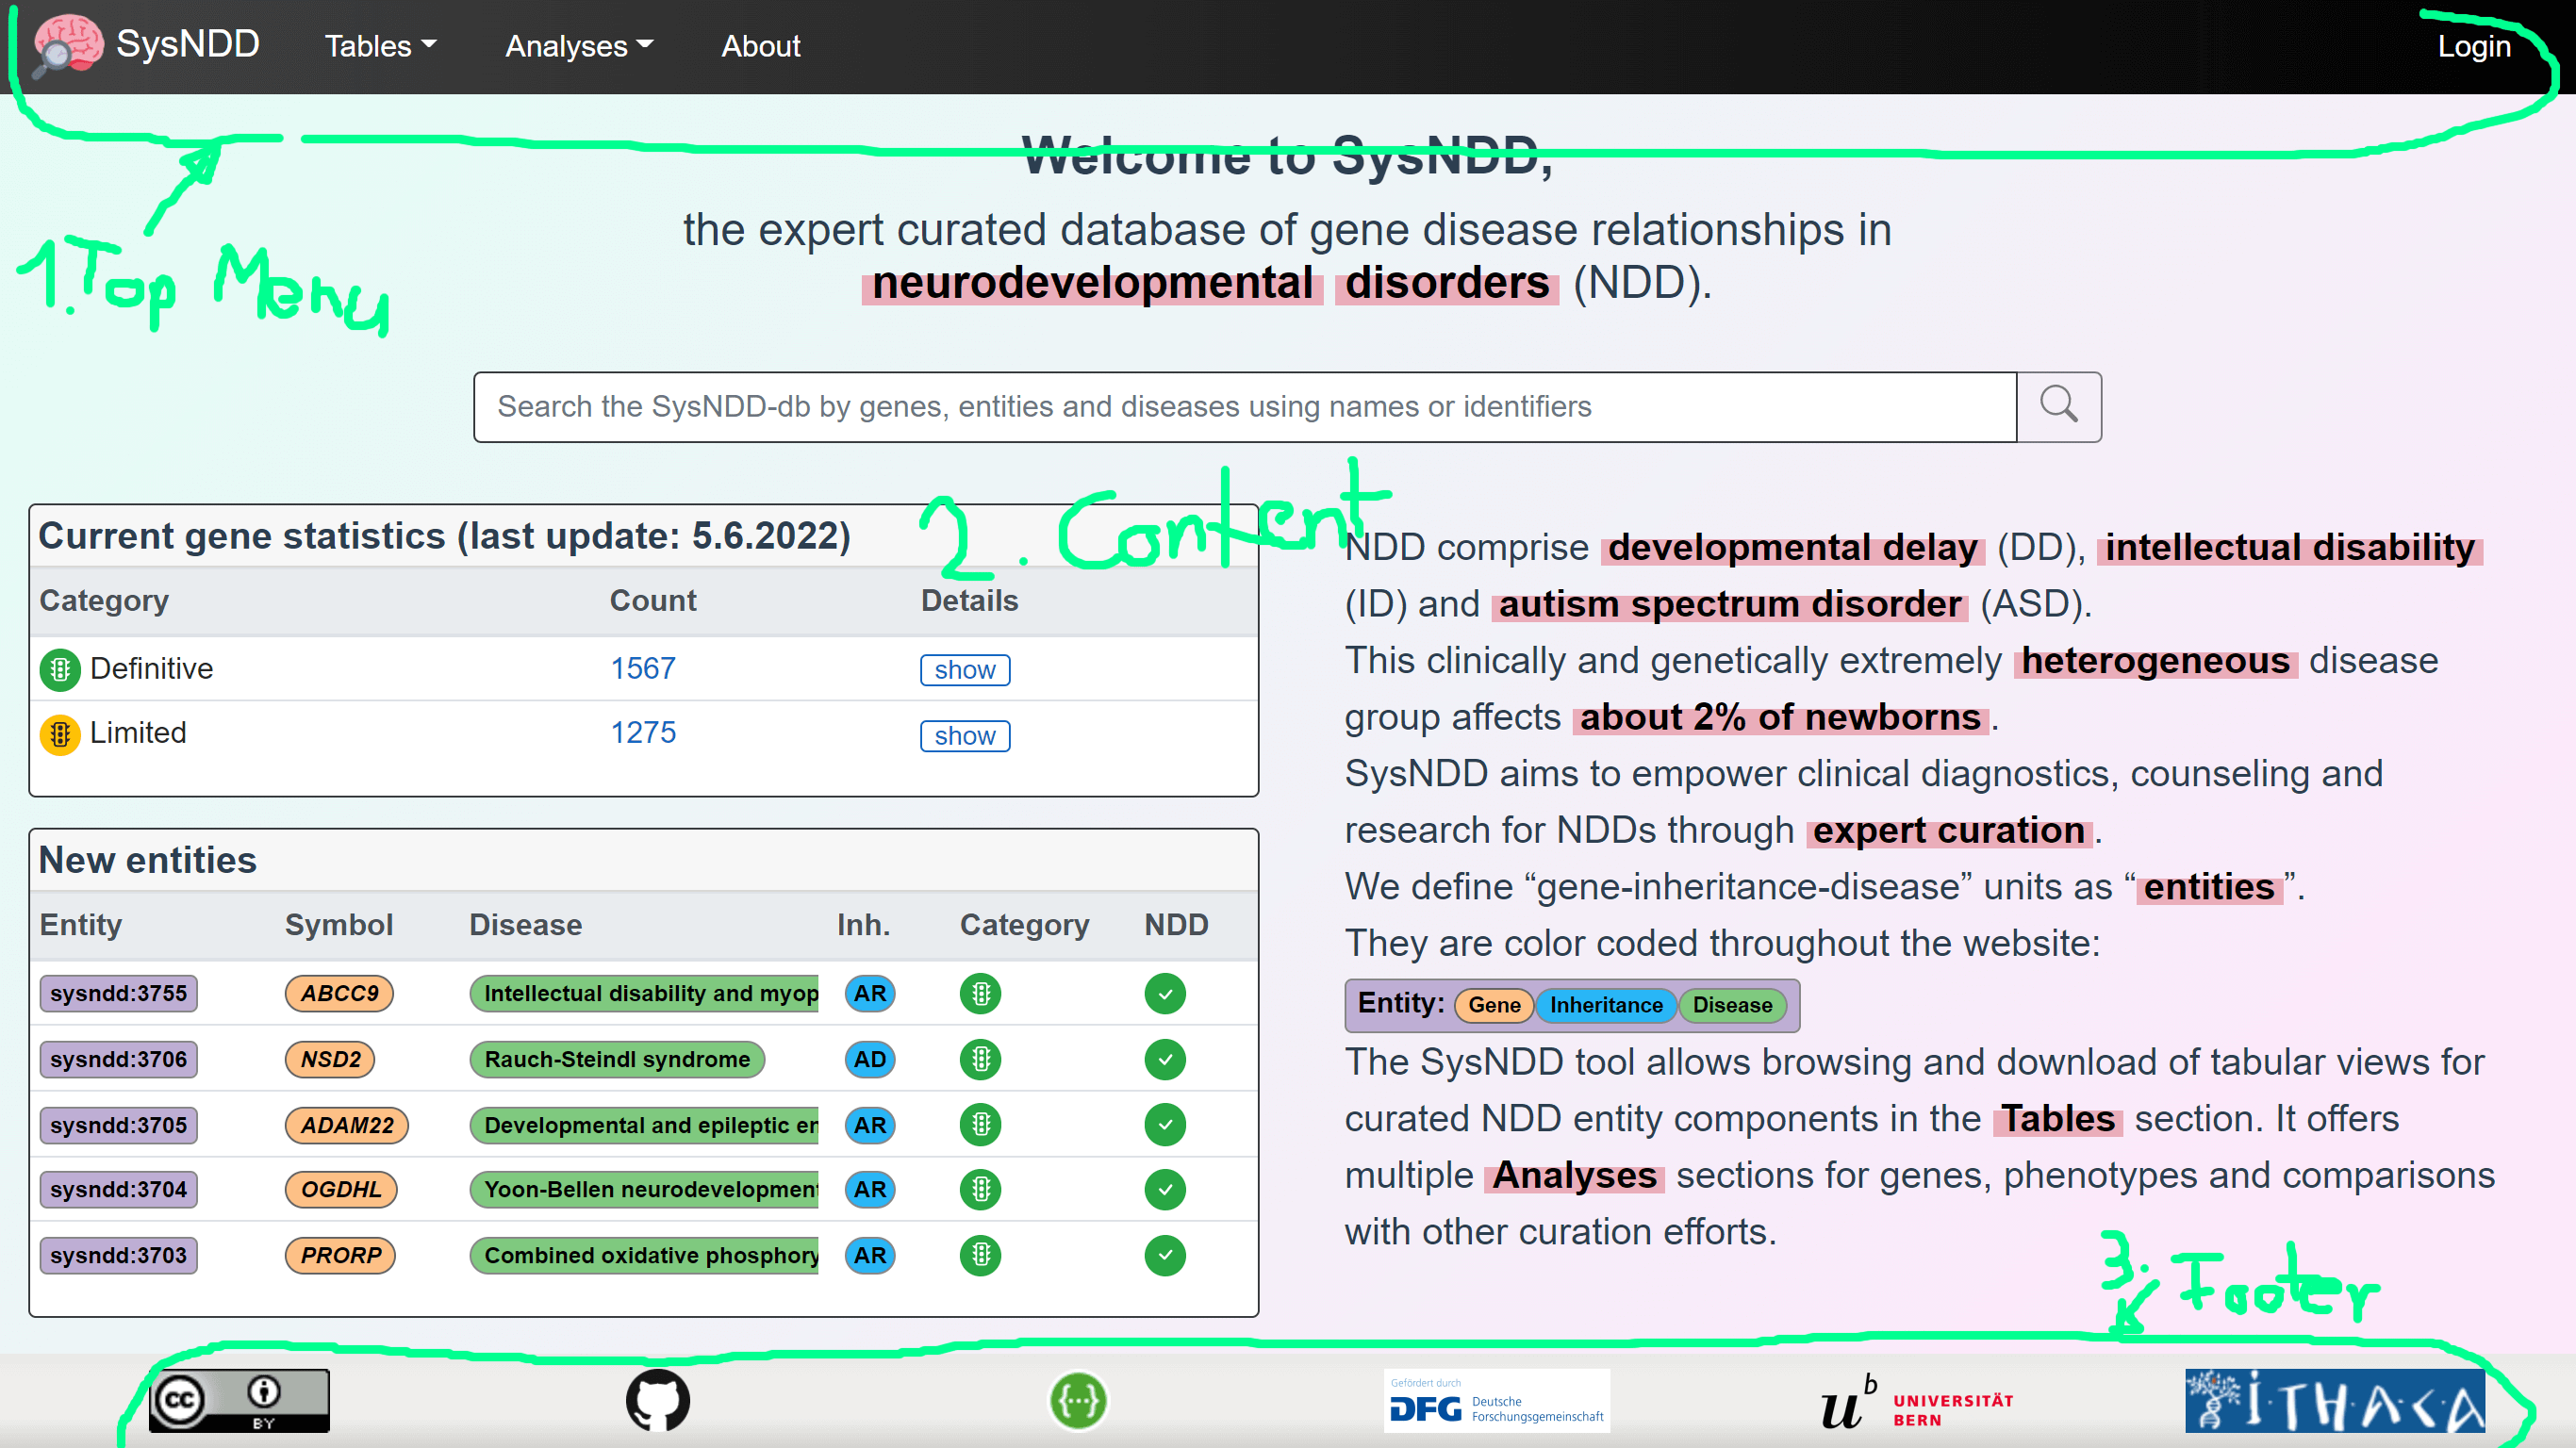
\includegraphics{./static/img/02_01-landing-page.png}
\caption{Landing page}
\end{figure}

The landing page content displays different elements to give a quick overview and allow fast navigation:

\begin{itemize}
\tightlist
\item
  a centered search input at the top,
\item
  a box (left side top) with current gene statistics divided by association category and inheritance patterns (Details),
\item
  a box (left side bottom) showing a table of the 5 last entities entered into the database,
\item
  an explanatory text on the right.
\end{itemize}

\hypertarget{main-navigation-menu}{%
\subsection{Main navigation menu}\label{main-navigation-menu}}

The main navigation allows quick access to all subpages.

The ``Tables'' button triggers a dropdown menu with links to:
- ``Entities'' table view
- ``Genes'' table view
- ``Phenotypes'' table view
- ``Panels table'' view

\begin{figure}
\centering
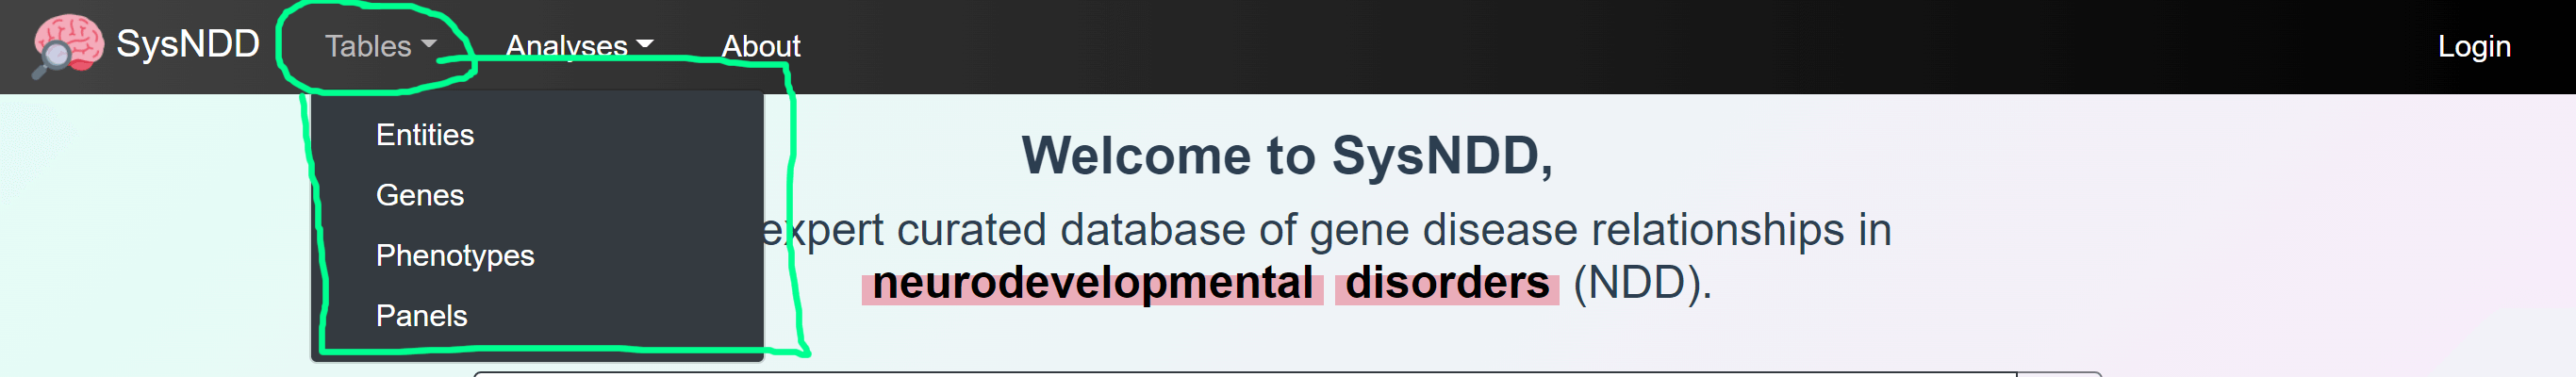
\includegraphics{./static/img/02_02-navigation-menu-tables.png}
\caption{Navigation menu tables}
\end{figure}

The ``Analyses'' button triggers a dropdown menu with links to:
- ``Compare curations'' view
- ``Correlate phenotypes'' view
- ``Entries over time'' view
- ``NDD Publications'' view
- ``Functional clusters'' view

\begin{figure}
\centering
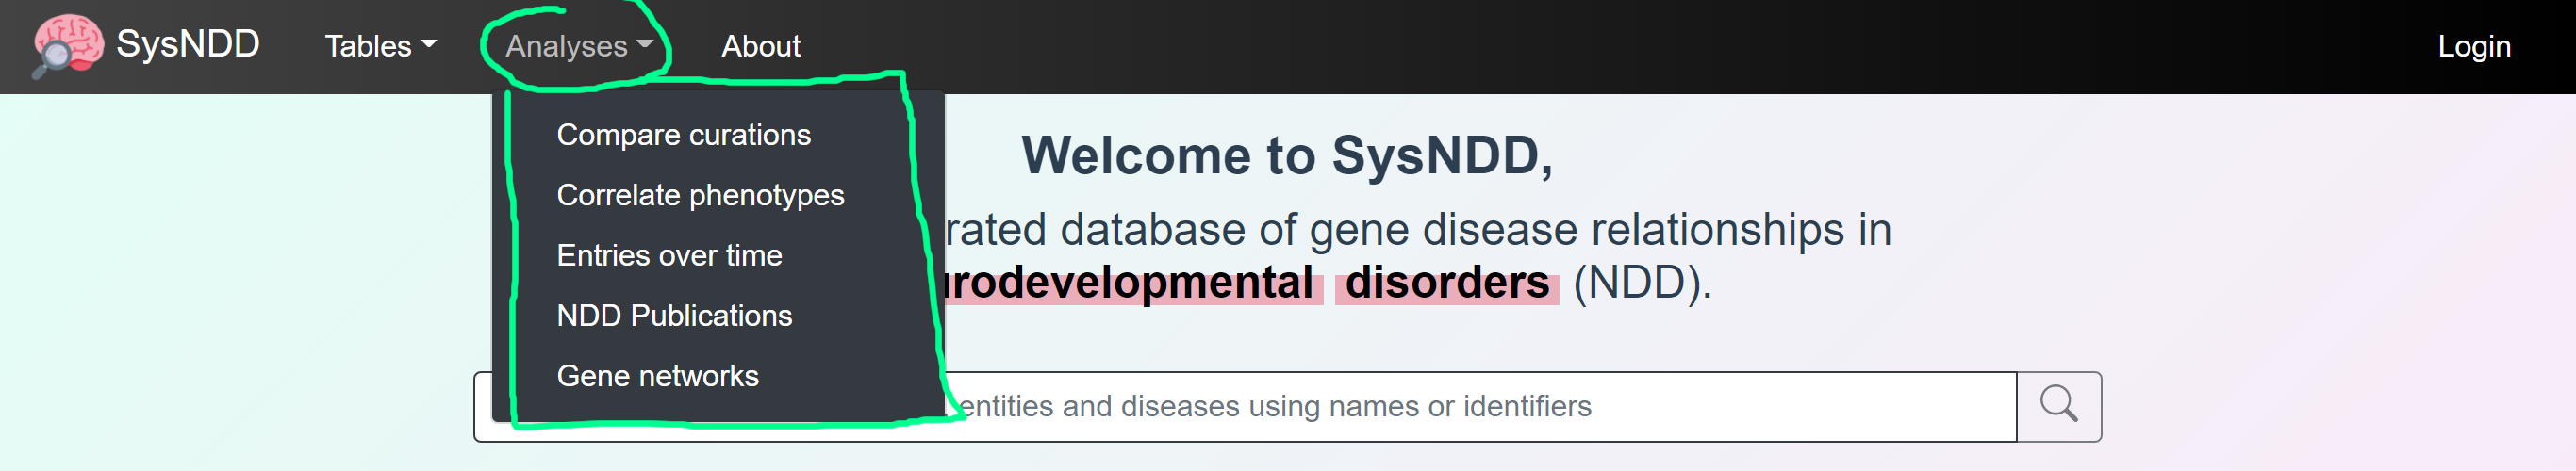
\includegraphics{./static/img/02_03-navigation-menu-analyses.png}
\caption{Navigation menu analyses}
\end{figure}

If not on the landing page, the navigation bar also contains a ``Search'' button which can show a search field on any page.

\begin{figure}
\centering
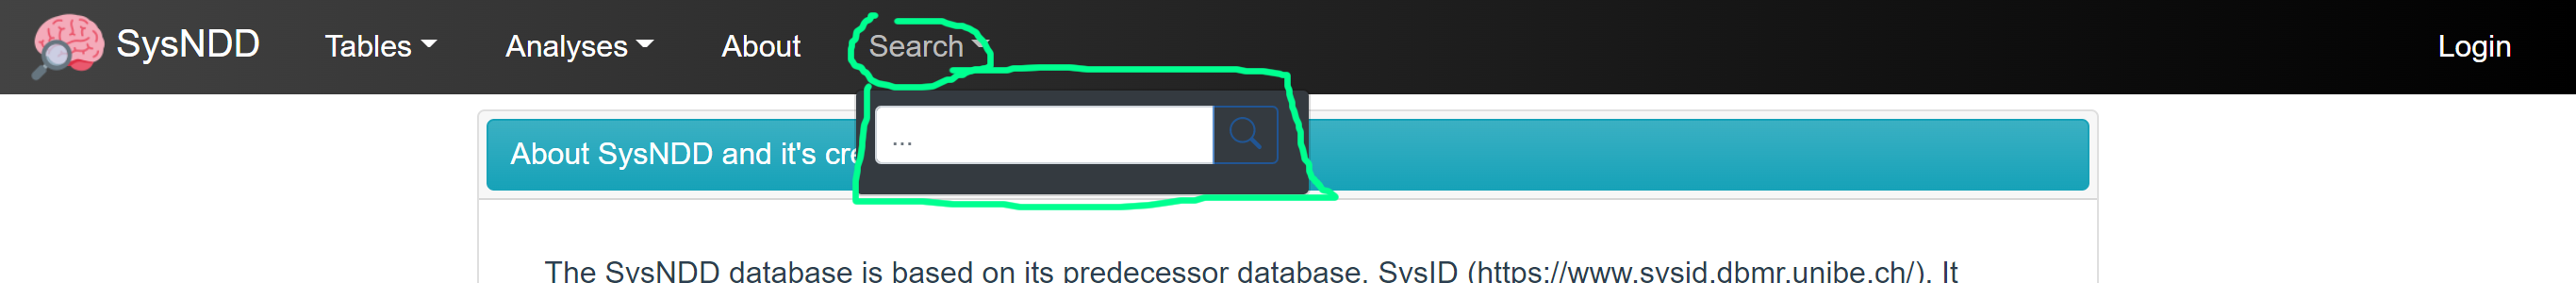
\includegraphics{./static/img/02_04-navigation-menu-search.png}
\caption{Navigation menu search}
\end{figure}

If not logged in the right side of the menu shows a button which directs to the Login page.
When logged in as a registered user the menu shows your username and additional links to page views depending on your user rights:

\begin{figure}
\centering
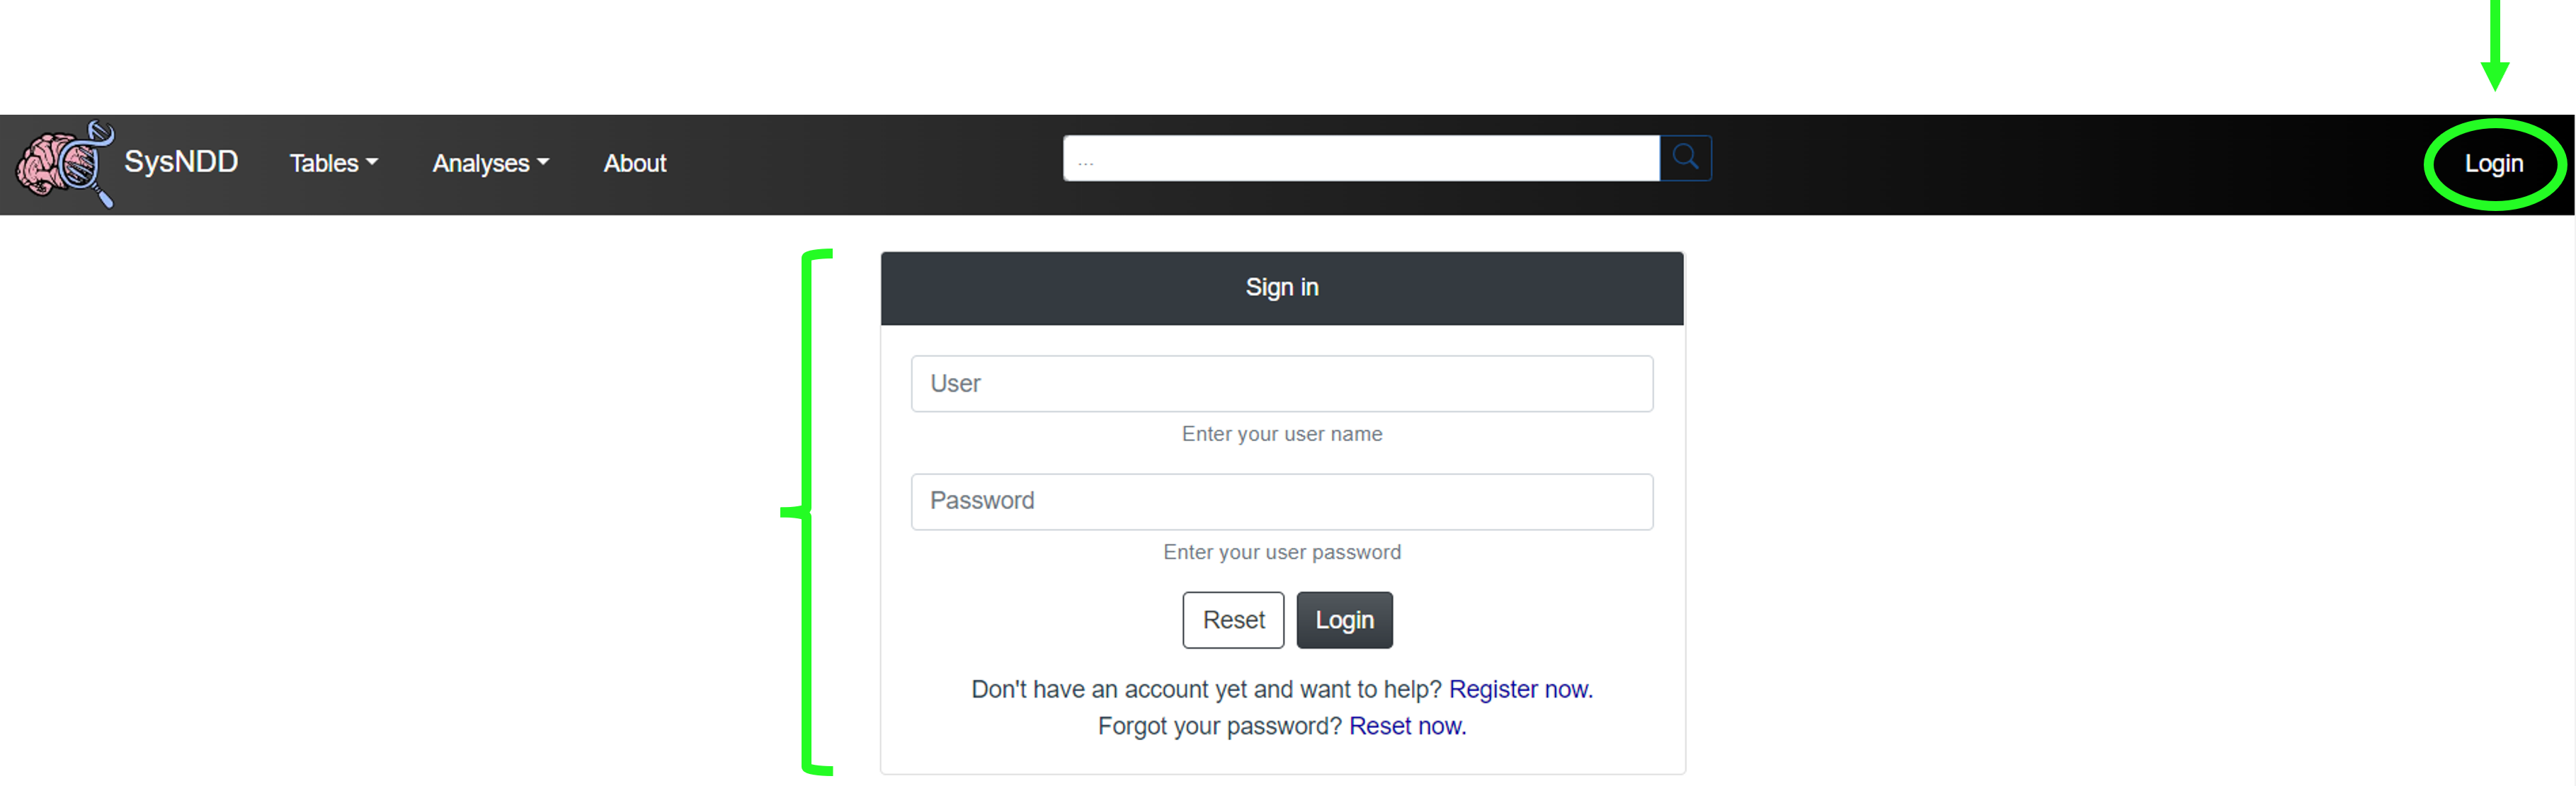
\includegraphics{./static/img/02_05-navigation-menu-login.png}
\caption{Navigation menu login}
\end{figure}

\hypertarget{footer-navigation-menu}{%
\subsection{Footer navigation menu}\label{footer-navigation-menu}}

The footer navigation shows pictures/ logos with links to:

\begin{enumerate}
\def\labelenumi{\arabic{enumi})}
\tightlist
\item
  the license applied to SysNDD
\item
  our GitHub repository
\item
  the SysNDD API view
\item
  the DFG funder website
\item
  the website of the University of Bern hosting our server
\item
  the ERN-ITHACA website
\end{enumerate}

\begin{figure}
\centering

\includegraphics{./static/img/02_06-footer-menu.png}
\caption{Footer navigation}
\end{figure}

\hypertarget{table-views}{%
\subsection{Table views}\label{table-views}}

We provide tabular representations with search, filtering, sorting and pagination functionality for different aspects of the entity concept.

\hypertarget{entities-table}{%
\subsubsection{Entities table}\label{entities-table}}

The Entities table is intended to provide an overview centered on the entity concept.

\begin{figure}
\centering
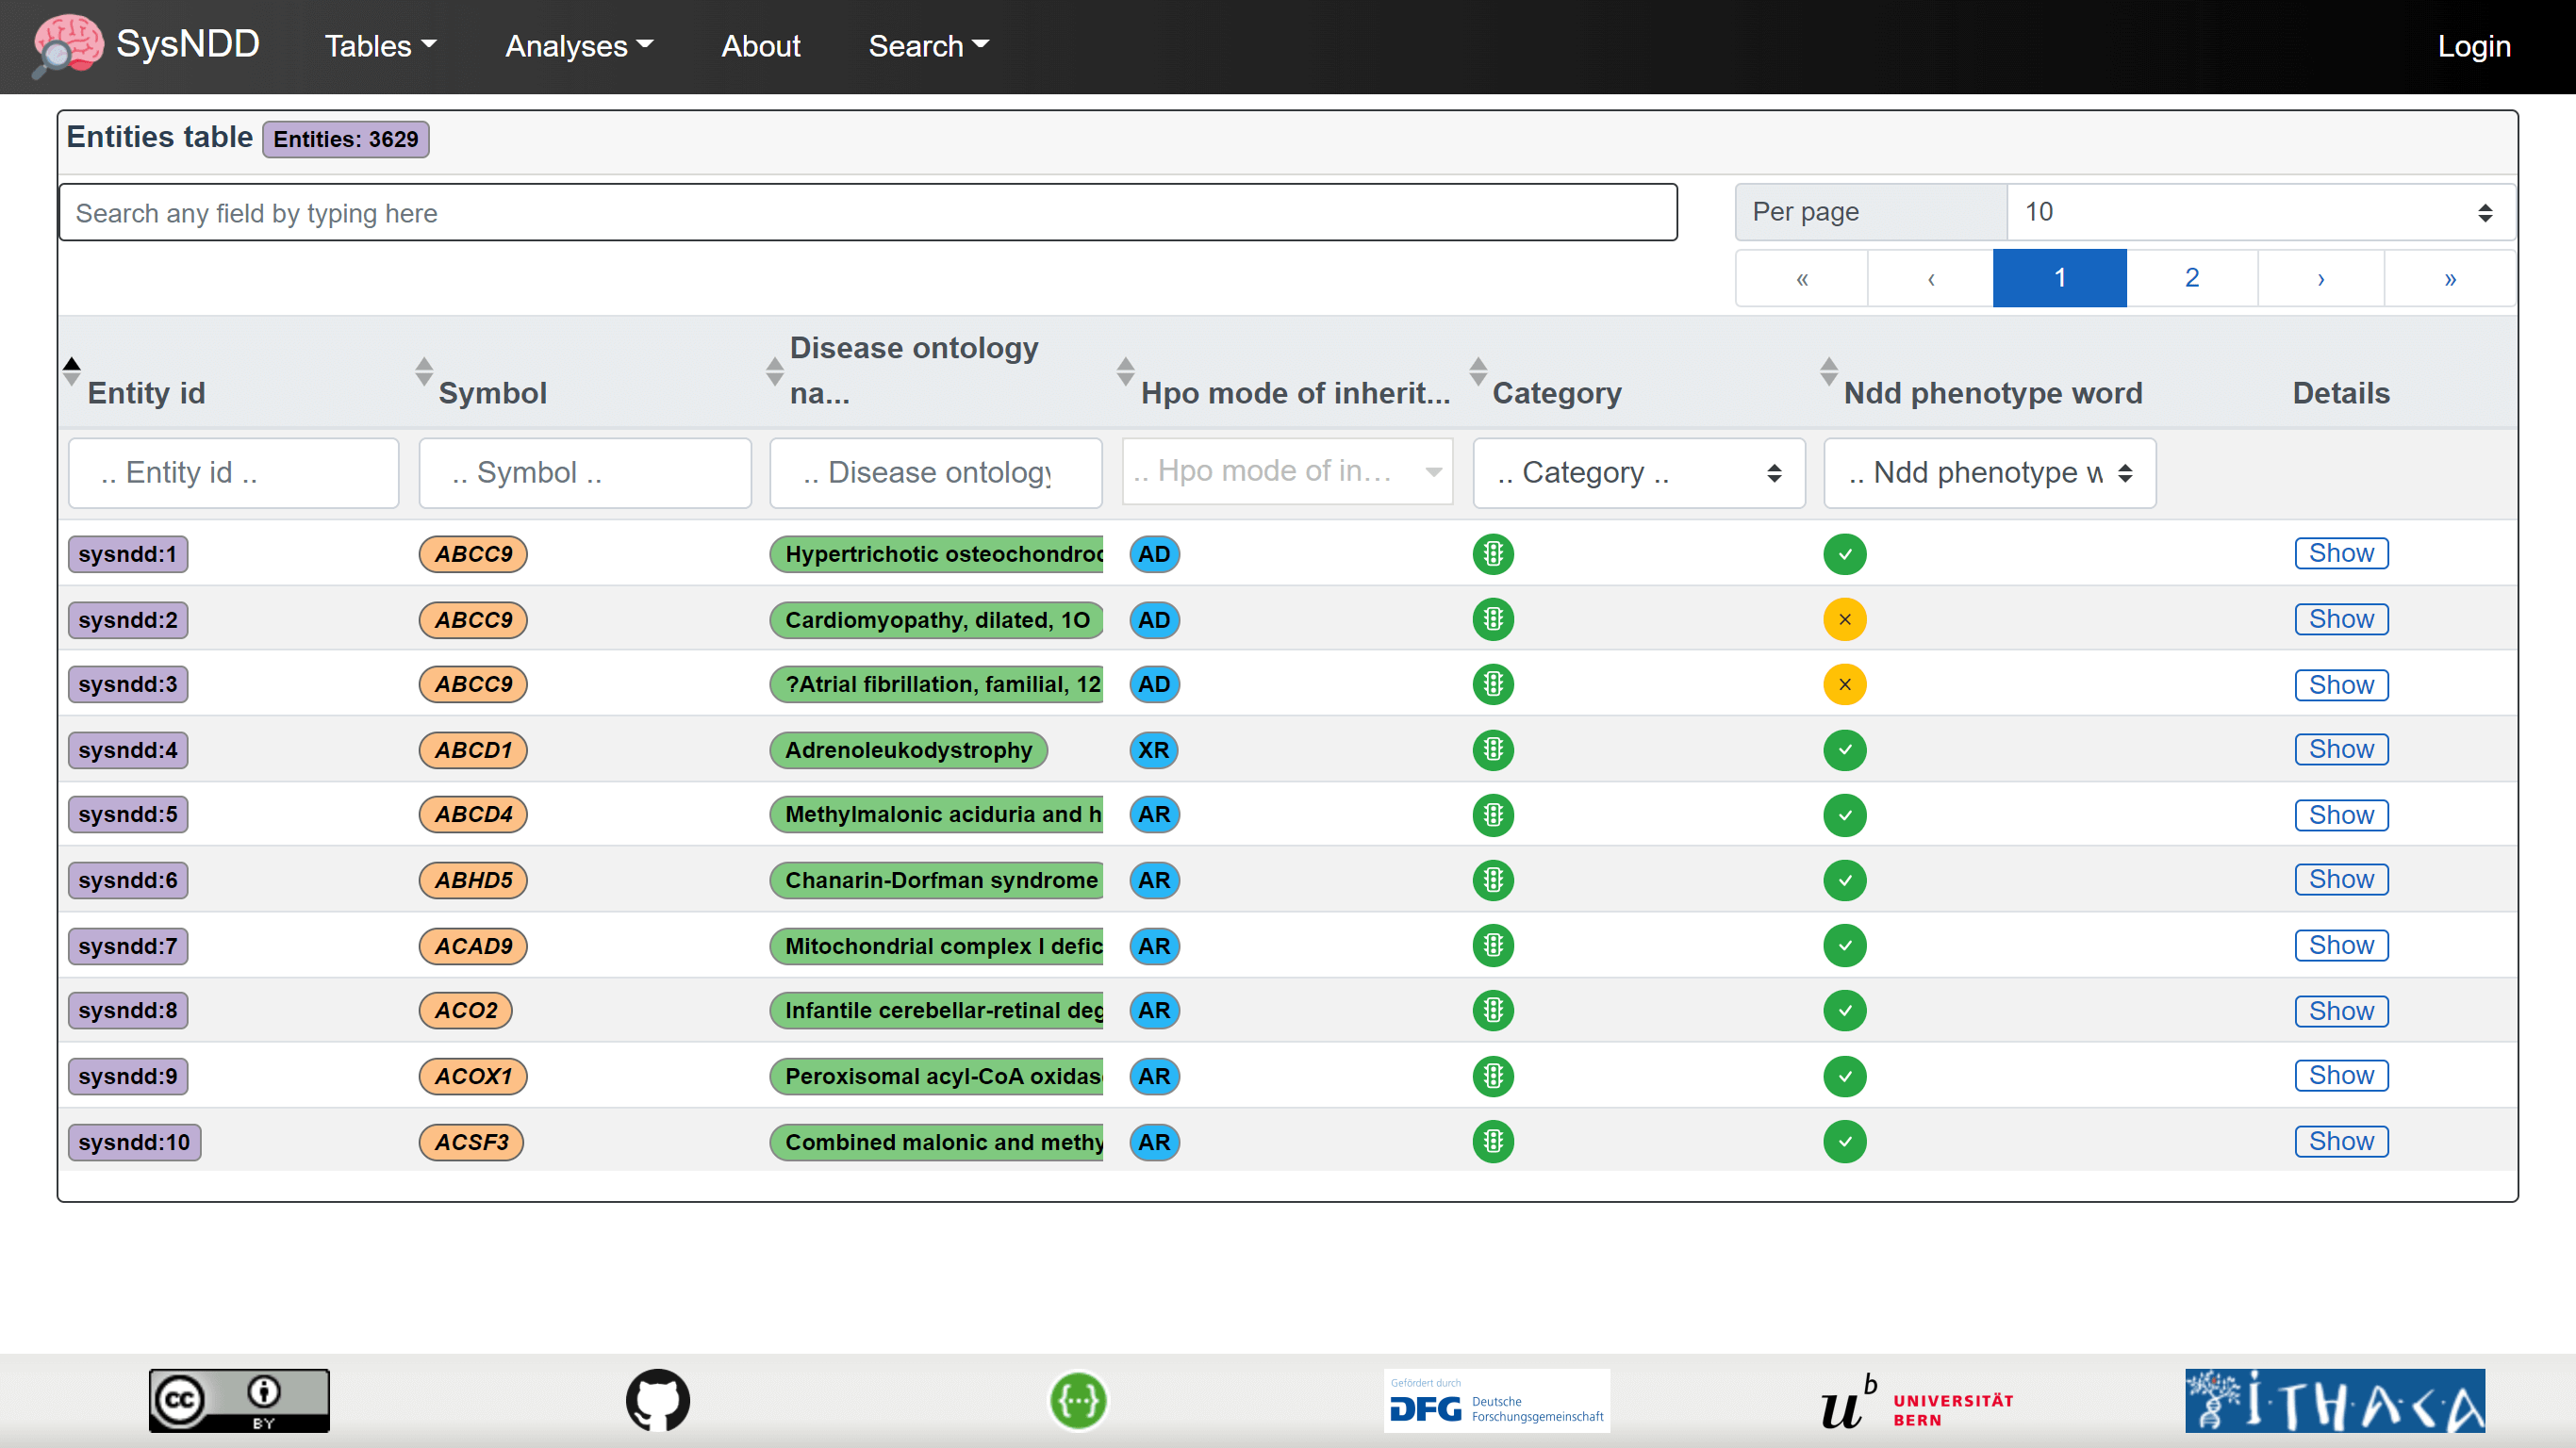
\includegraphics{./static/img/02_07-sysndd.dbmr.unibe.ch_Entities.png}
\caption{Entities view}
\end{figure}

\hypertarget{genes-table}{%
\subsubsection{Genes table}\label{genes-table}}

The Genes table is intended to provide a gene-centered overview.

\begin{figure}
\centering
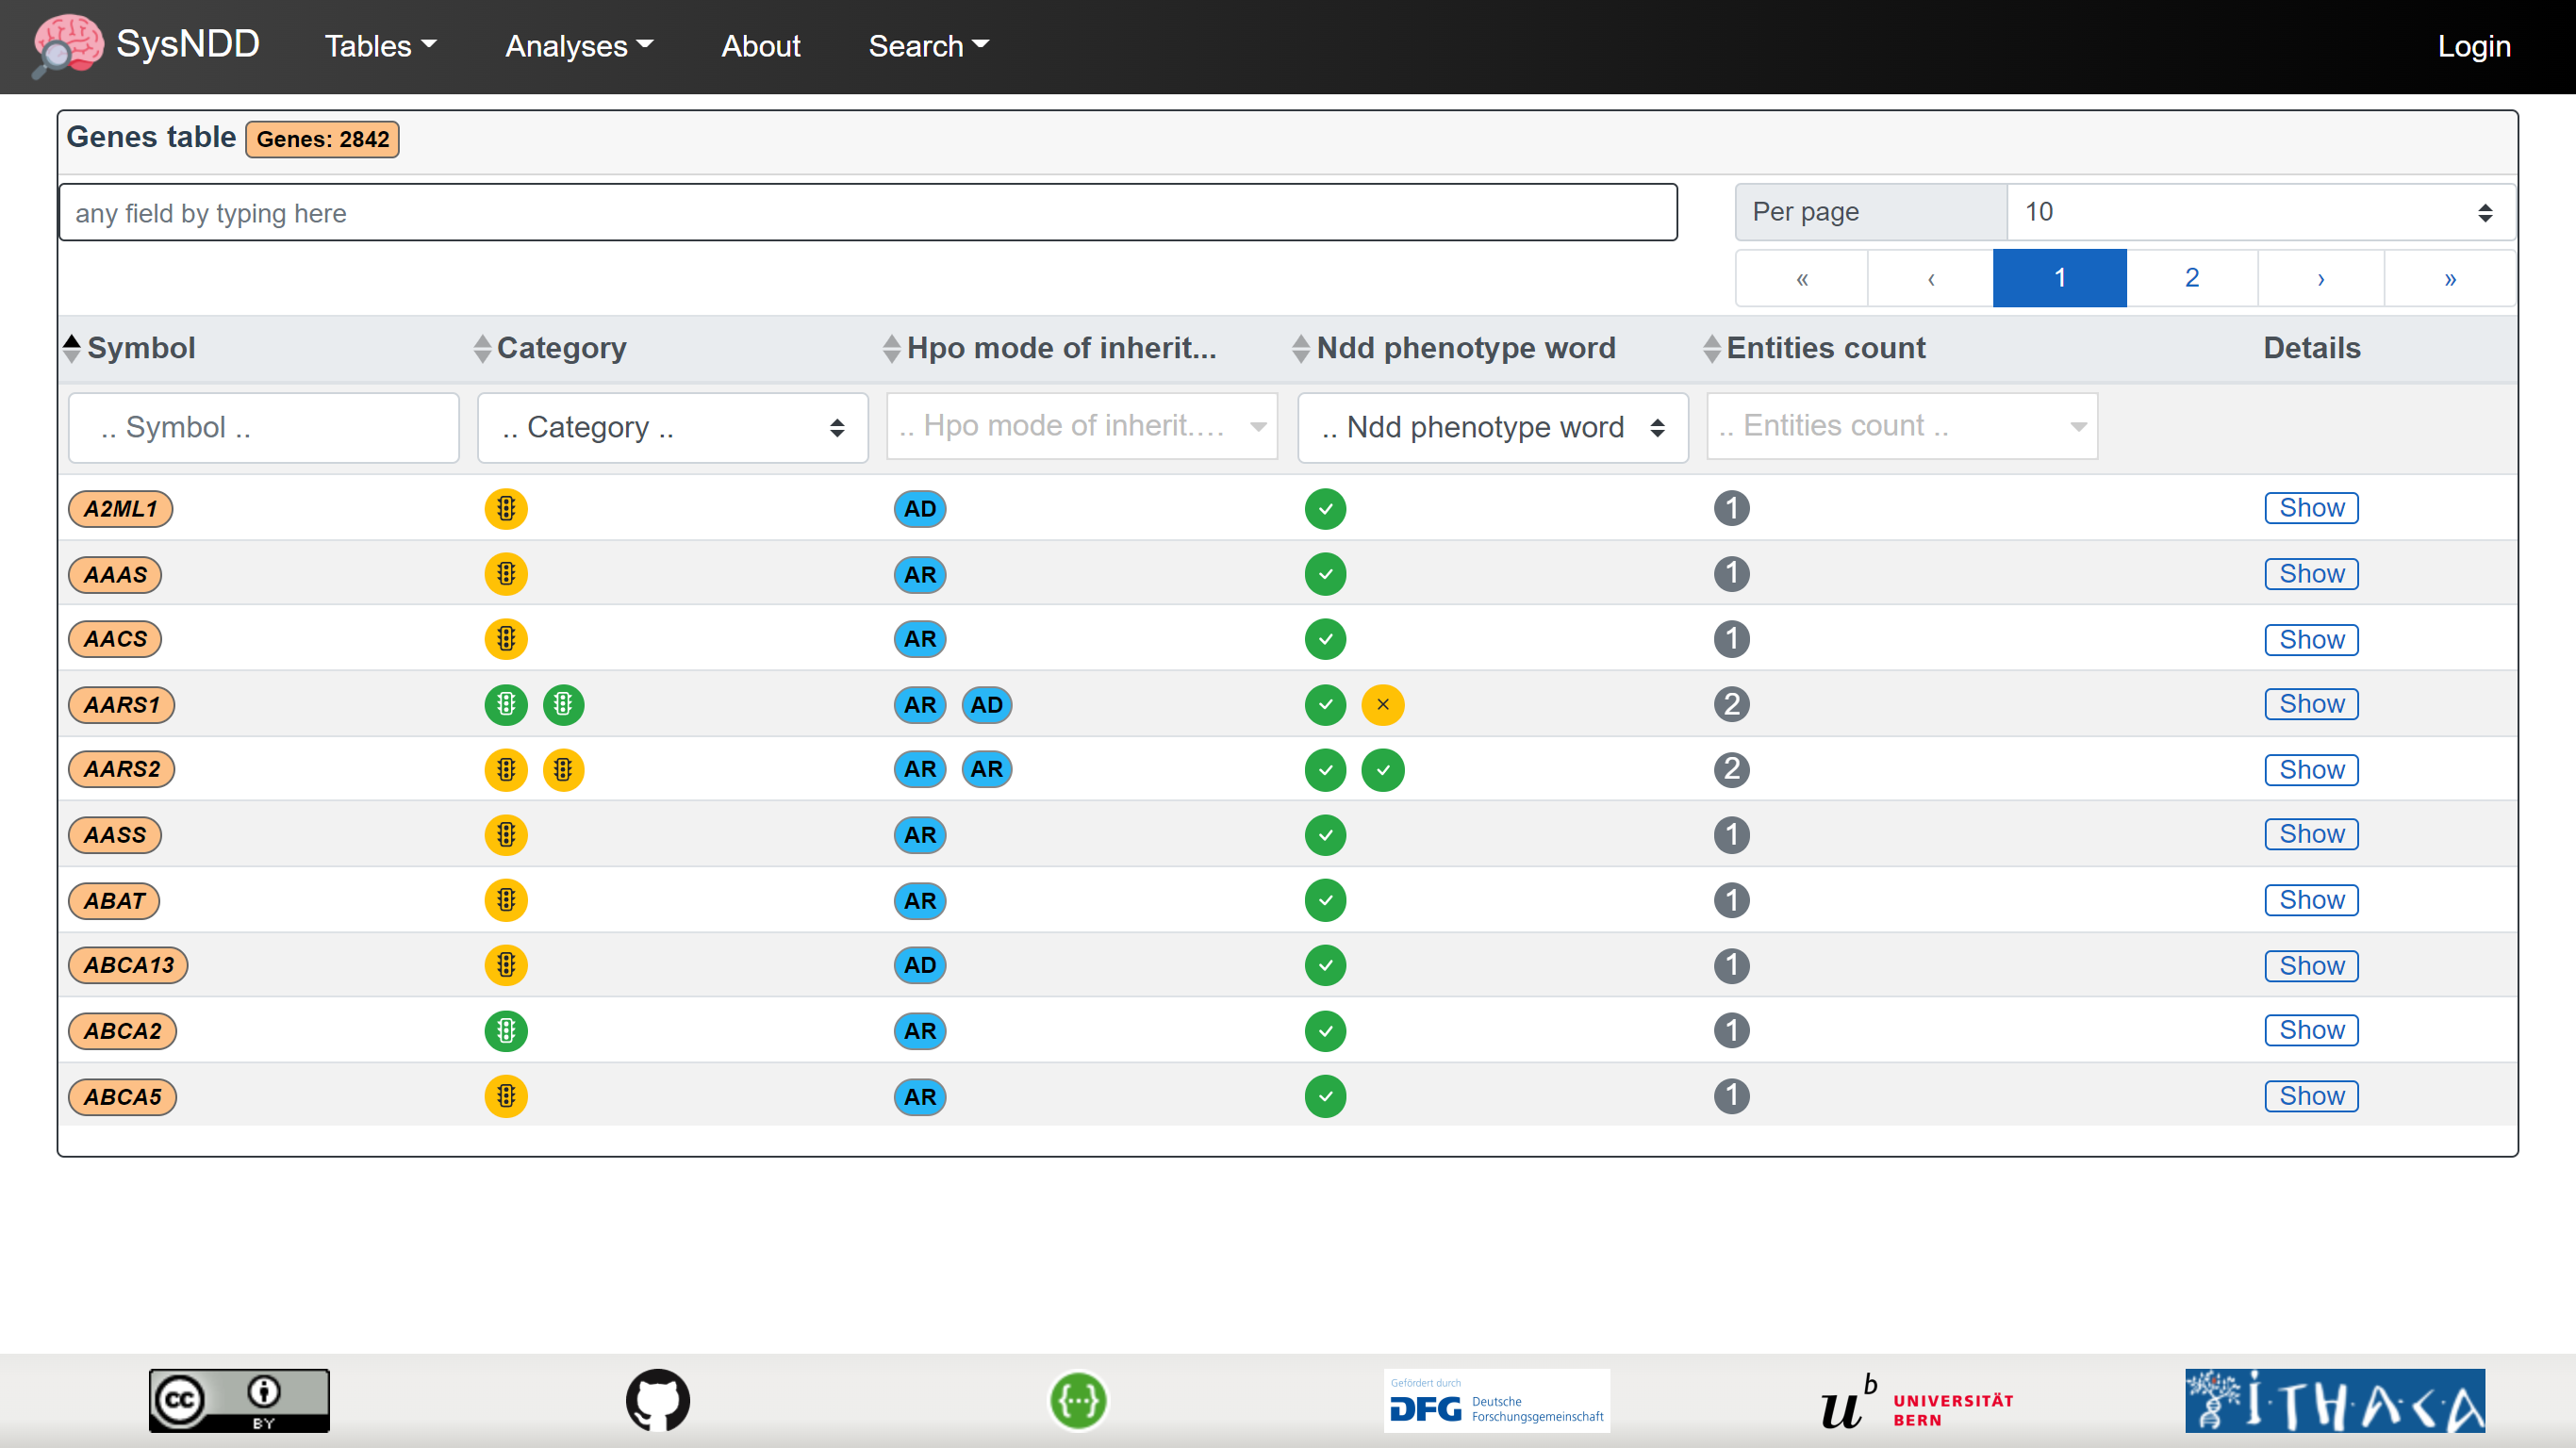
\includegraphics{./static/img/02_08-sysndd.dbmr.unibe.ch_Genes.png}
\caption{Genes view}
\end{figure}

\hypertarget{phenotypes-table}{%
\subsubsection{Phenotypes table}\label{phenotypes-table}}

The Phenotypes table provides the possibility to filter for phenotype combinations annotated to the entities.

\begin{figure}
\centering
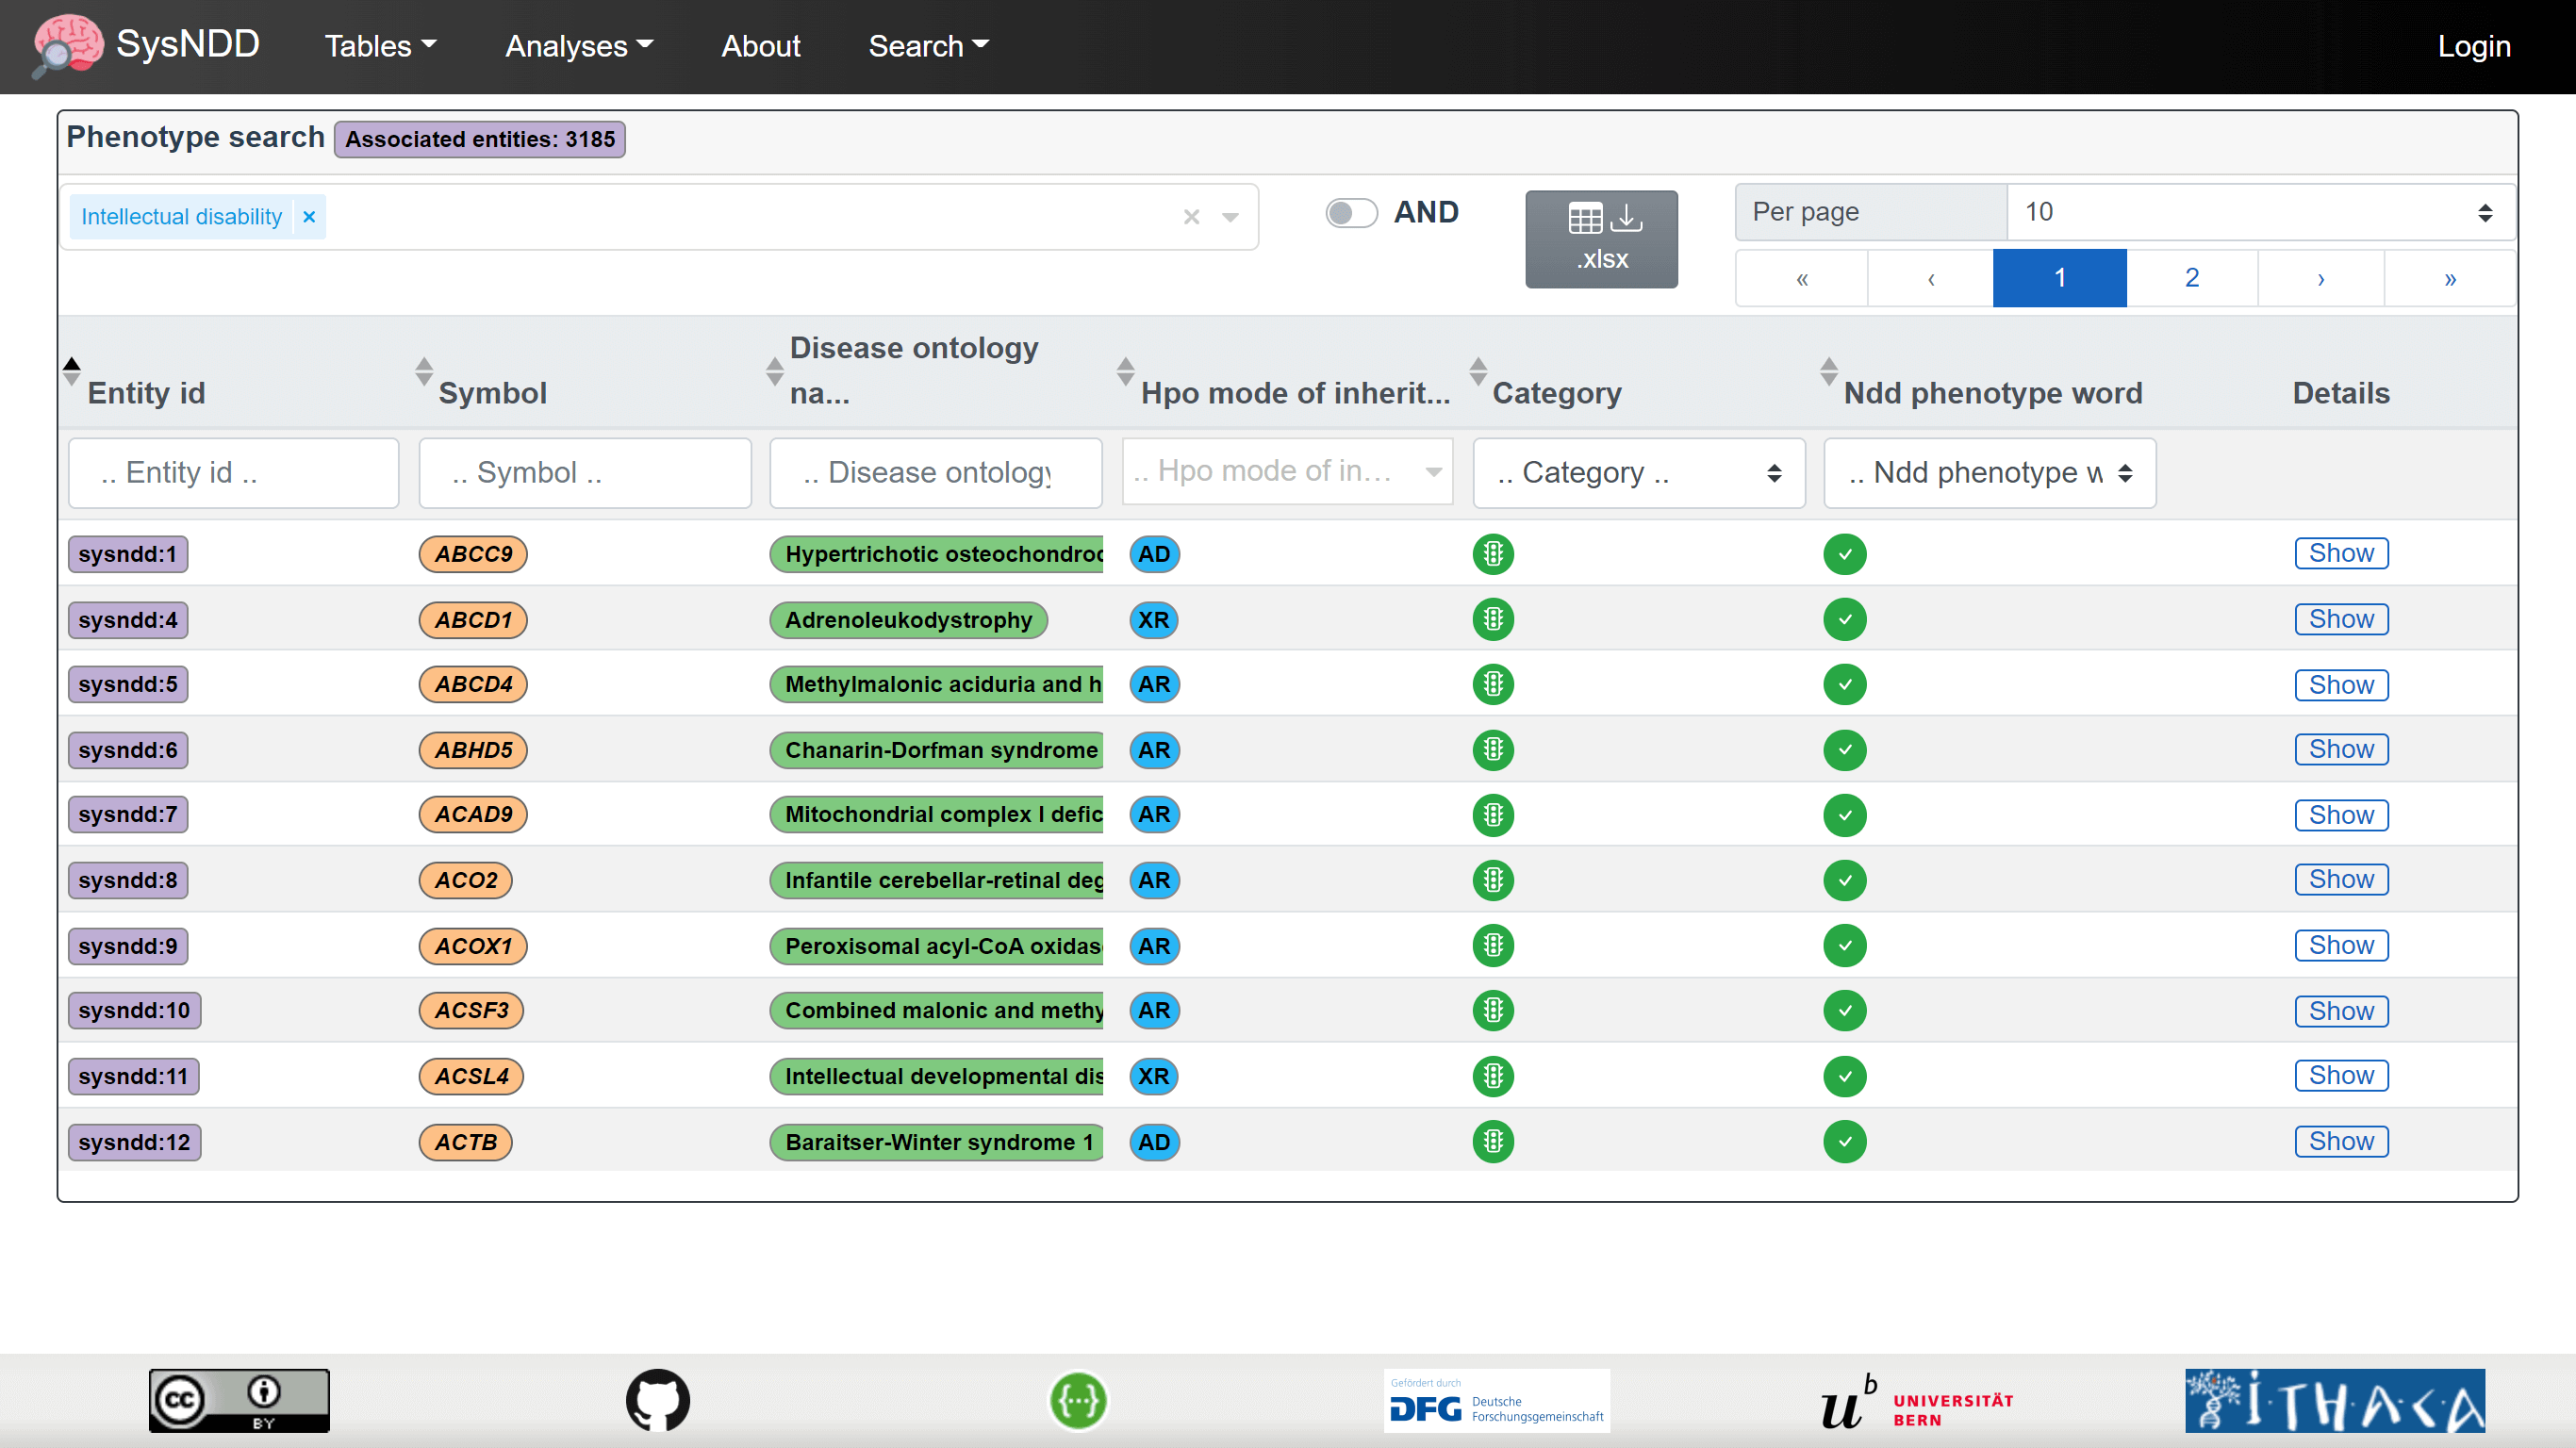
\includegraphics{./static/img/02_09-sysndd.dbmr.unibe.ch_Phenotypes.png}
\caption{Phenotypes view}
\end{figure}

The ``AND/ OR'' switch allows the user to change the logik how phenotype combinations are requested:

\begin{itemize}
\tightlist
\item
  AND: only entities having all selected phenoytpes annotated are shown.
\item
  OR: all entities having any of the selected phenoytpes annotated are shown.
\end{itemize}

\hypertarget{panels-table}{%
\subsubsection{Panels table}\label{panels-table}}

The Panels table is intended for users to be able to create lists of NDD-associated genes. Additionally, the columns in the lists can be configured.
Finally, the configuration can be downloaded as Excel file with information on the exact query in the meta sheet and the requested information in the ``data'' sheet.
These files can then be used as ``virtual panels'' to filter genetic variants derived from high-throughput sequencing in external analysis tools.

\begin{figure}
\centering
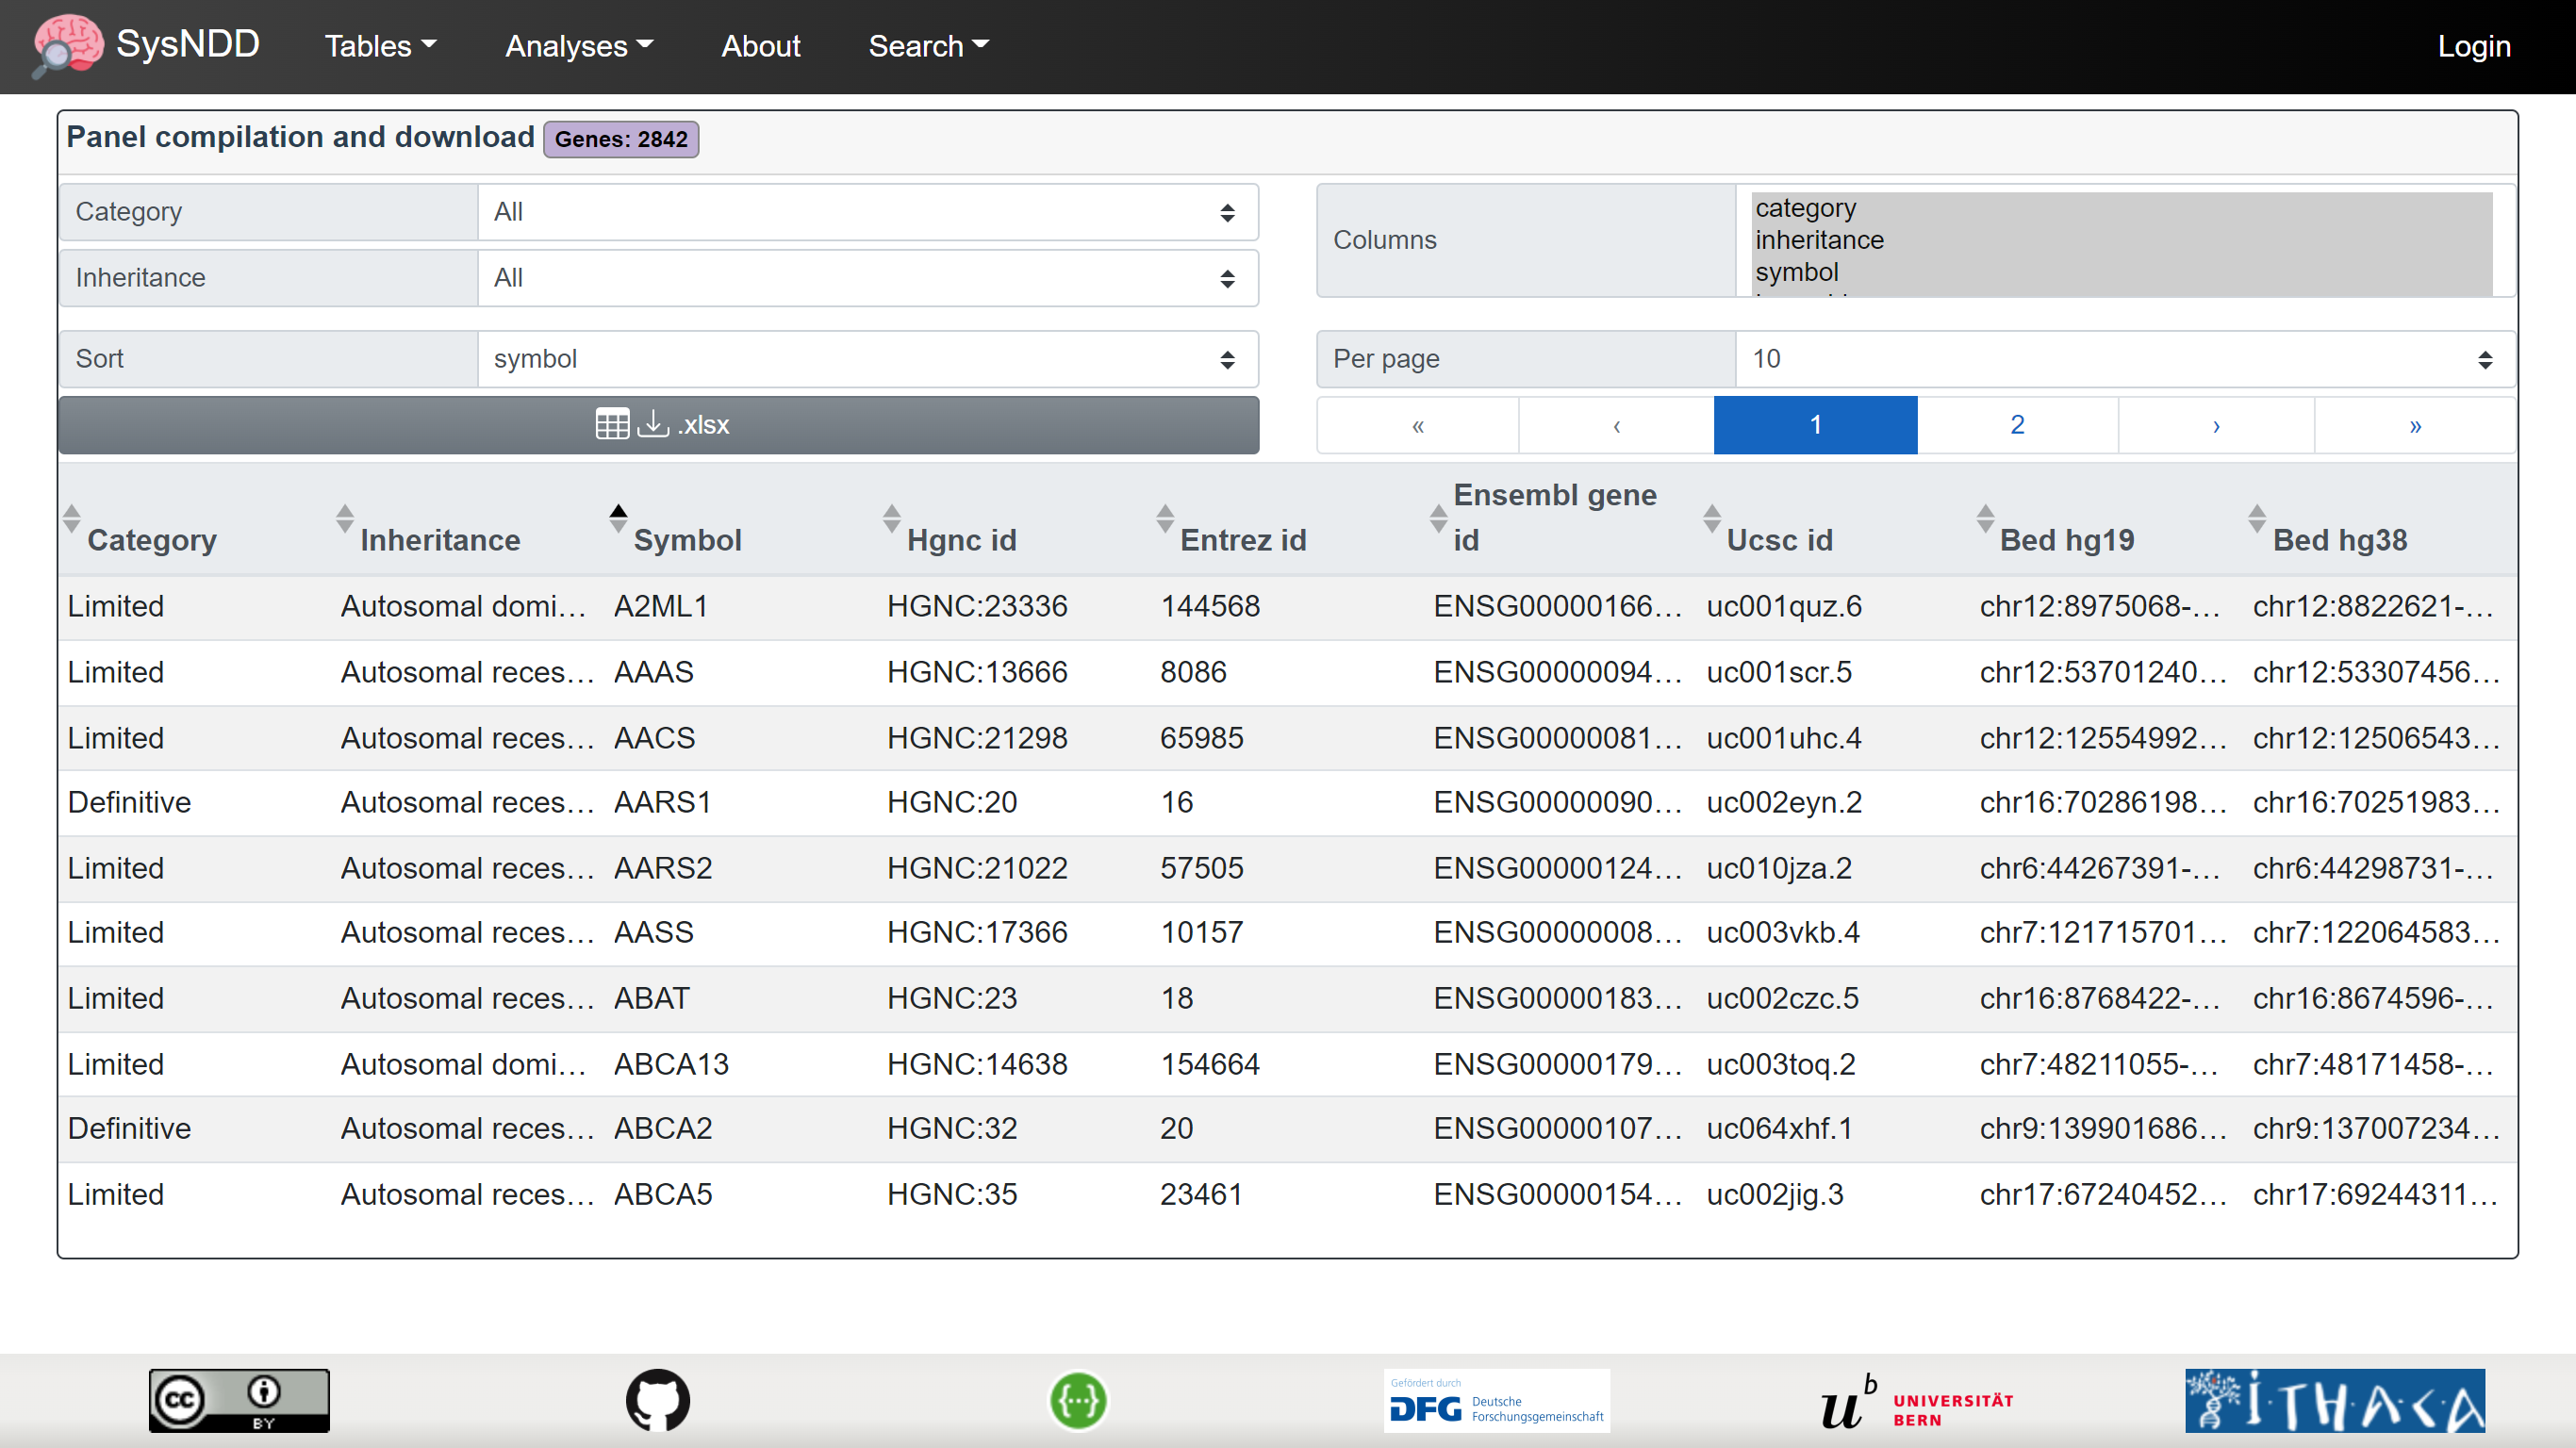
\includegraphics{./static/img/02_10-sysndd.dbmr.unibe.ch_Panels.png}
\caption{Panels view}
\end{figure}

\hypertarget{single-entry-pages}{%
\subsection{Single entry pages}\label{single-entry-pages}}

\hypertarget{entity}{%
\subsubsection{Entity}\label{entity}}

\hypertarget{gene}{%
\subsubsection{Gene}\label{gene}}

\hypertarget{ontology}{%
\subsubsection{Ontology}\label{ontology}}

\hypertarget{analyses-views}{%
\subsection{Analyses views}\label{analyses-views}}

\hypertarget{compare-curations}{%
\subsubsection{Compare curations}\label{compare-curations}}

\hypertarget{correlate-phenotypes}{%
\subsubsection{Correlate phenotypes}\label{correlate-phenotypes}}

\hypertarget{entries-over-time}{%
\subsubsection{Entries over time}\label{entries-over-time}}

\hypertarget{ndd-publications}{%
\subsubsection{NDD Publications}\label{ndd-publications}}

\hypertarget{functional-clusters}{%
\subsubsection{Functional clusters}\label{functional-clusters}}

\hypertarget{about-page}{%
\subsection{About page}\label{about-page}}

The About page contains general information about the project, its creators, funding, updates, and how to find help.

\hypertarget{login-page}{%
\subsection{Login page}\label{login-page}}

The Login page shows a simple form with inputs for the \textbf{(1)} user name and their \textbf{(2)} password, \textbf{(3)} buttons to reset the form and \textbf{(4)} links to registration and password reset.

\begin{figure}
\centering
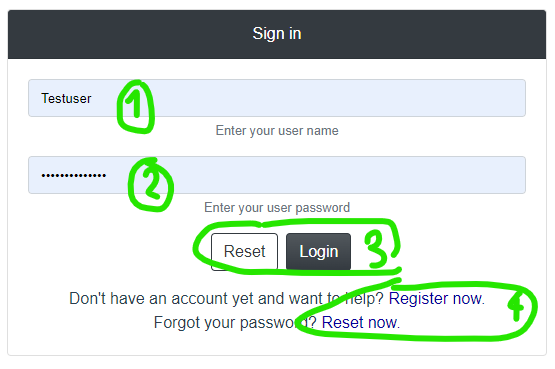
\includegraphics{./static/img/02_16-login-modal.png}
\caption{Login modal}
\end{figure}

\hypertarget{register-user-page}{%
\subsubsection{Register user page}\label{register-user-page}}

This page can be used to apply for a SysNDD account by entering following information:

\begin{enumerate}
\def\labelenumi{\arabic{enumi})}
\tightlist
\item
  desired username
\item
  institutional E-mail
\item
  ORCID identifier
\item
  First name
\item
  Family name
\item
  description of your interest in SysNDD and why you want to participate in the curation effort
\end{enumerate}

and \textbf{(7)} accepting the terms of use.

The \textbf{(8)} buttons allow resetting or submitting the form.

\begin{figure}
\centering
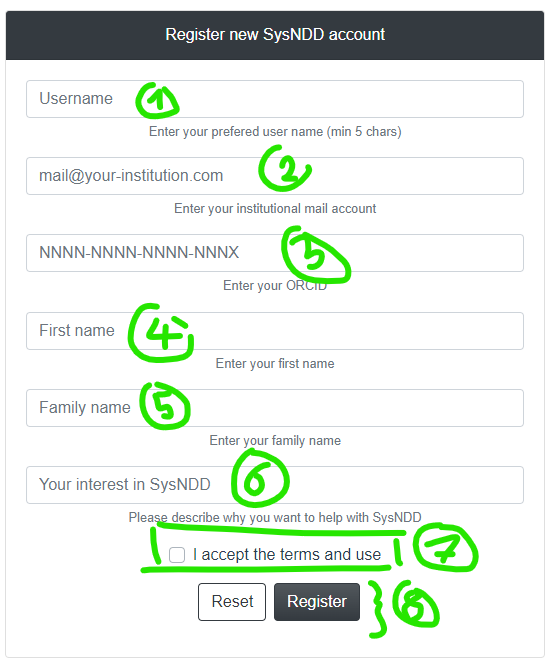
\includegraphics{./static/img/02_17-register-modal.png}
\caption{Register modal}
\end{figure}

Upon submission the curator status users will receive a mail to review your application. After your application has been confirmed you will receive a mail with your login information and instructions.

\hypertarget{reset-password-page}{%
\subsubsection{Reset password page}\label{reset-password-page}}

The form on this page allows users who forgot their password to reset this by enetering the E-mail tehy registered with.

\begin{figure}
\centering
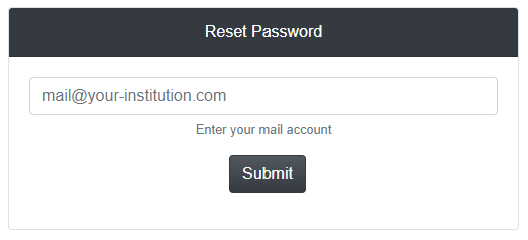
\includegraphics{./static/img/02_18-password-reset-modal.png}
\caption{Reset modal}
\end{figure}

Upon submission the E-mail account will receive a message with a one-time link allowing the user to enter a new password.

\hypertarget{mobile-website}{%
\subsection{Mobile website}\label{mobile-website}}

The Vue.js framework enables native cross platform development. Together with the Bootstrap CSS library this enables the SysNDD web app to seamlessly integrate on smaller mobile screens.

\begin{figure}
\centering
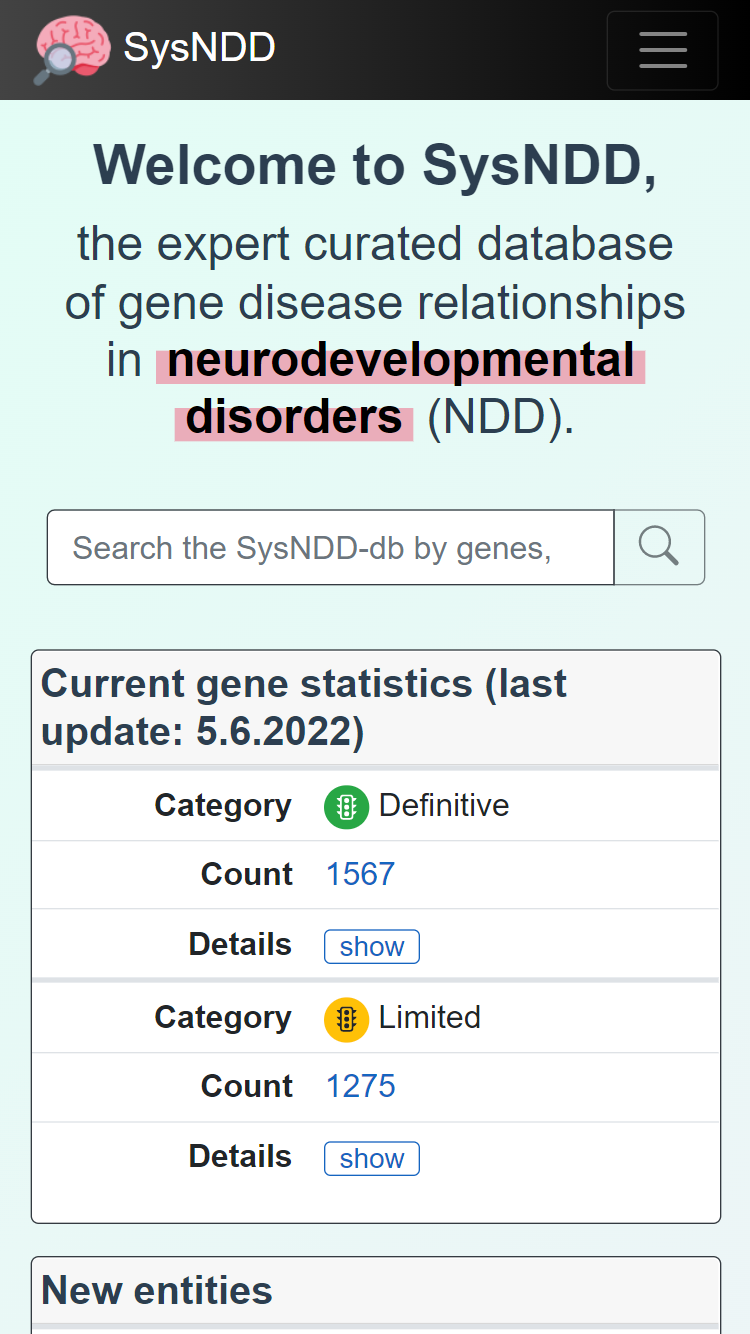
\includegraphics{./static/img/02_19-mobile-site.png}
\caption{Mobile site}
\end{figure}

The layout breaks to mobile view at 768 pixels width and minimizes the navigation and footer menus:

\begin{figure}
\centering
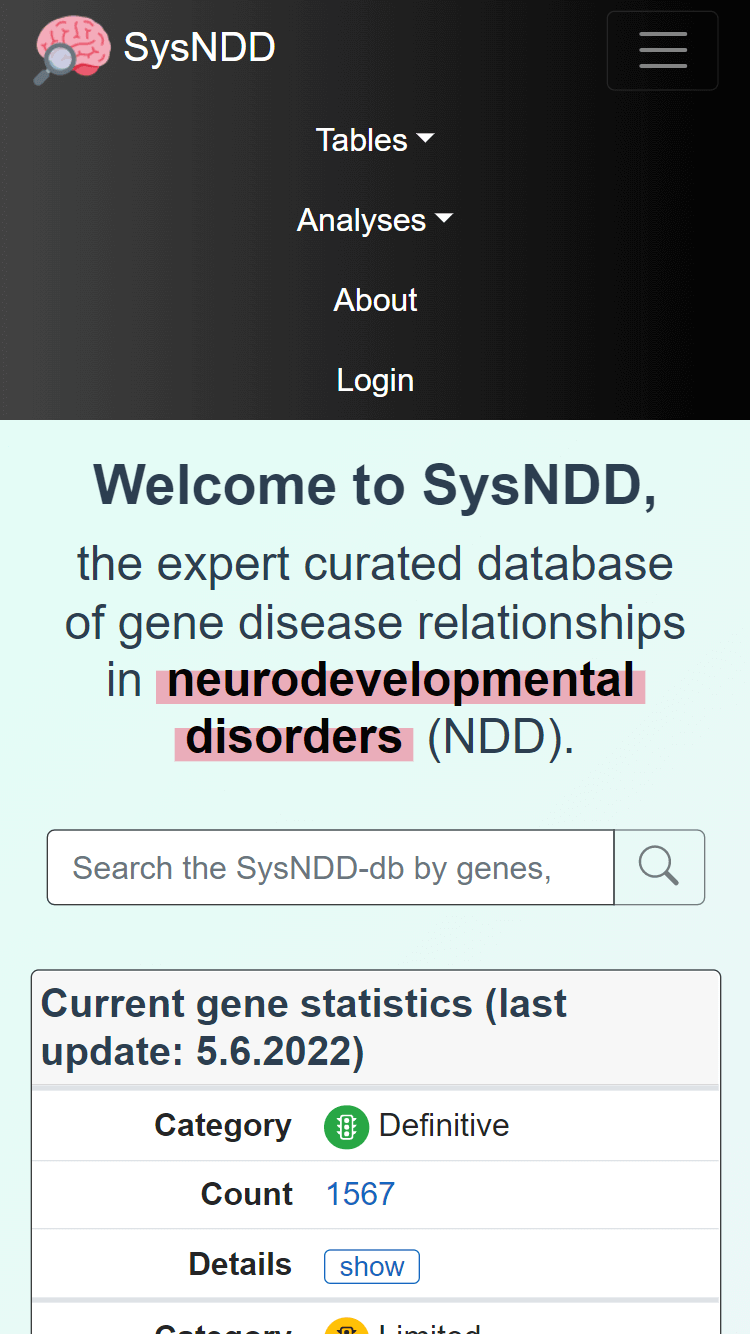
\includegraphics{./static/img/02_20-mobile-navbar.png}
\caption{Mobile navbar}
\end{figure}

\begin{figure}
\centering
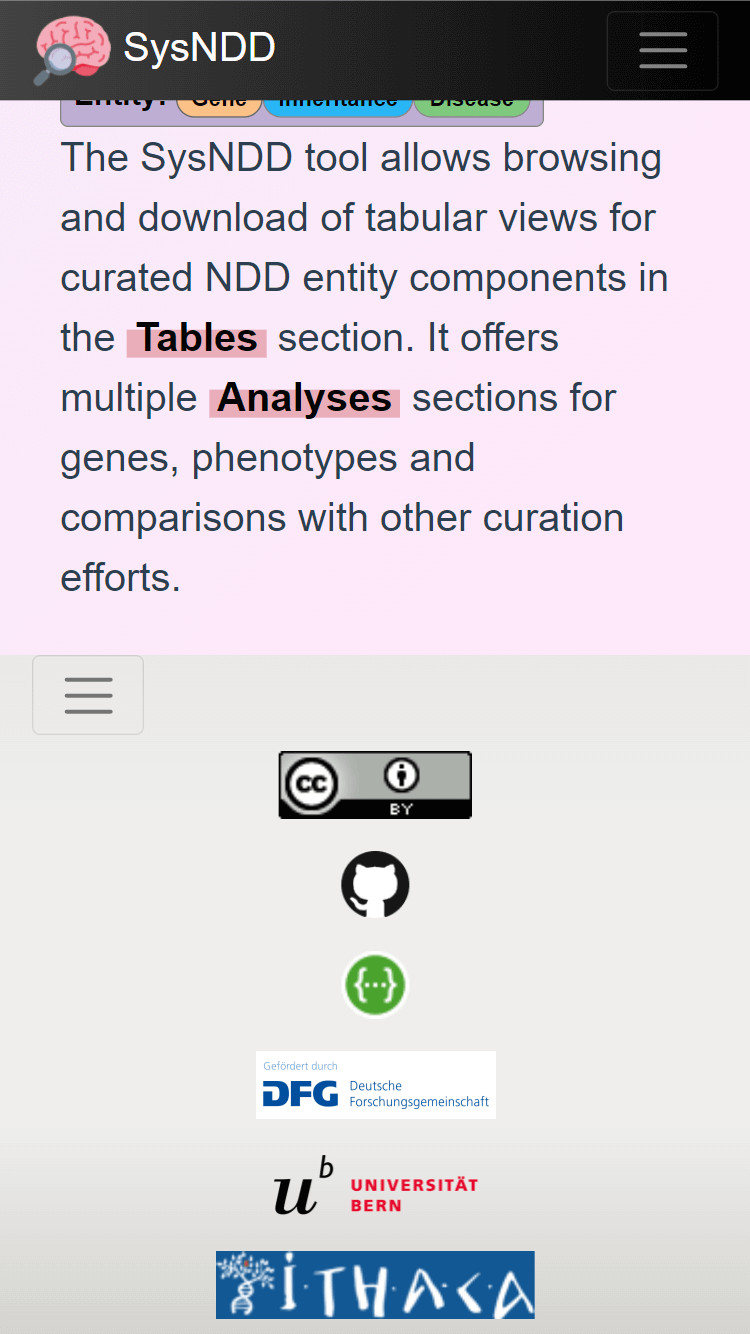
\includegraphics{./static/img/02_21-mobile-footer.png}
\caption{Mobile footer}
\end{figure}

All tables in mobile views break to a stacked view (column names becoem first column in a cell and values second column) to best use display space:

\begin{figure}
\centering
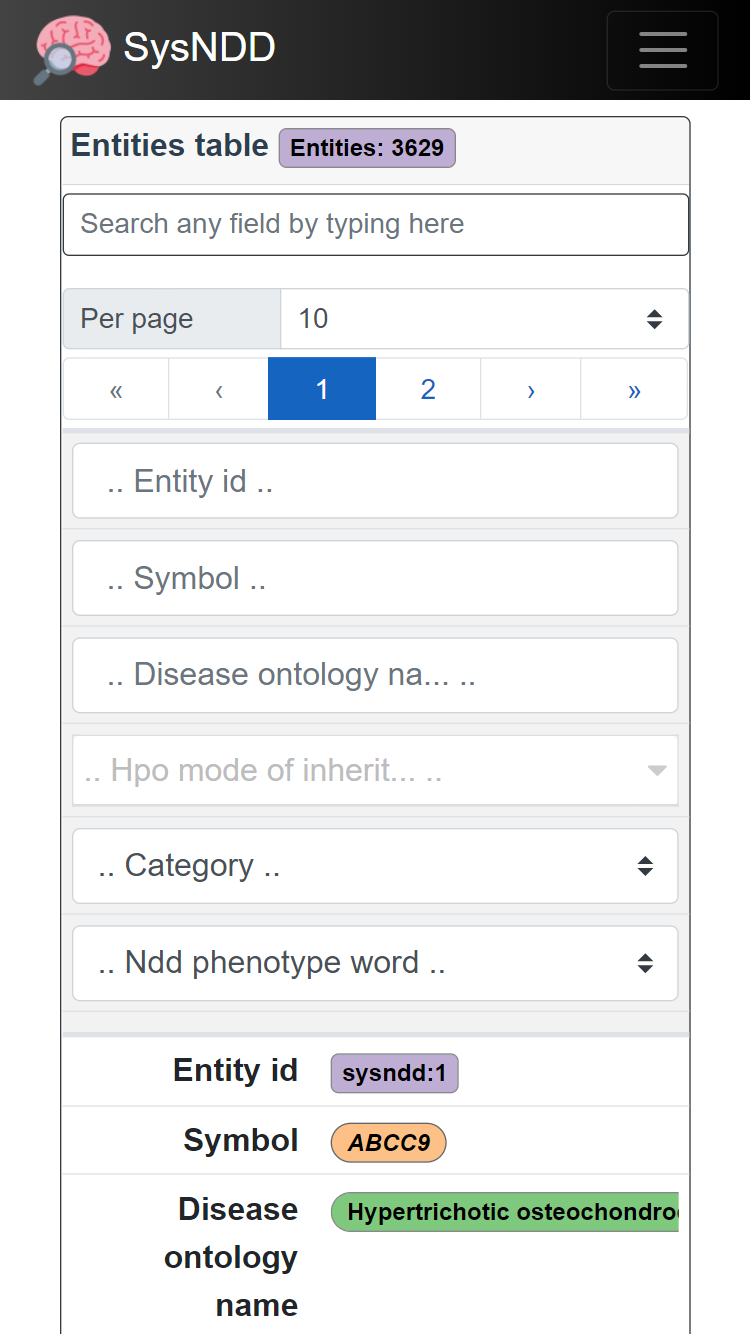
\includegraphics{./static/img/02_22-mobile-stacked-table.png}
\caption{Stacked table}
\end{figure}

The table controls and search inputs are further dispalyed at the top in this view.

The analyses pages on mobile pages are best viewed in landscape mode:

\begin{figure}
\centering
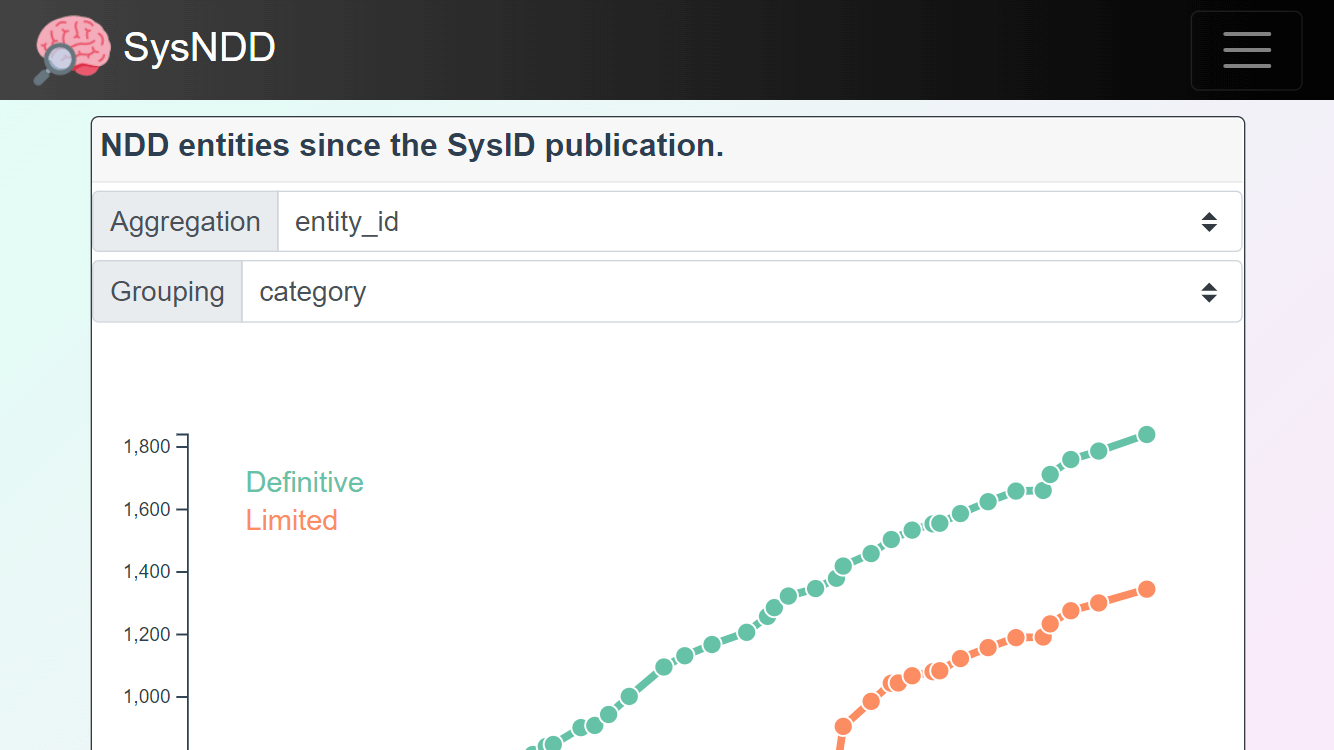
\includegraphics{./static/img/02_23-mobile-analyses-landscape.png}
\caption{Landscape mode}
\end{figure}

\hypertarget{progressive-web-app-pwa}{%
\subsection{Progressive Web App (PWA)}\label{progressive-web-app-pwa}}

The SysNDD web app can also be installed on mobile devices using the Progressive Web App (\href{https://en.wikipedia.org/wiki/Progressive_web_application}{PWA}) technology.
This is supported in all Chromium-based modern browsers (Chrome, Edge, Opera, etc.) on all common operating systems (Windows, Linux, maxOS and Android).
Additionally new Safari versions on iOS show some support for PWA.

PWAs are faster because they cache files. They offer more screen space for the app. Future integrations of this feature in SysNDD will enable offline use.

To install the PWA on Android devices follow these steps:

\textbf{1)} Visit the SysNDD website at \url{https://sysndd.dbmr.unibe.ch/}. You will see a message offering to add the PWA to your home screen:

\begin{figure}
\centering
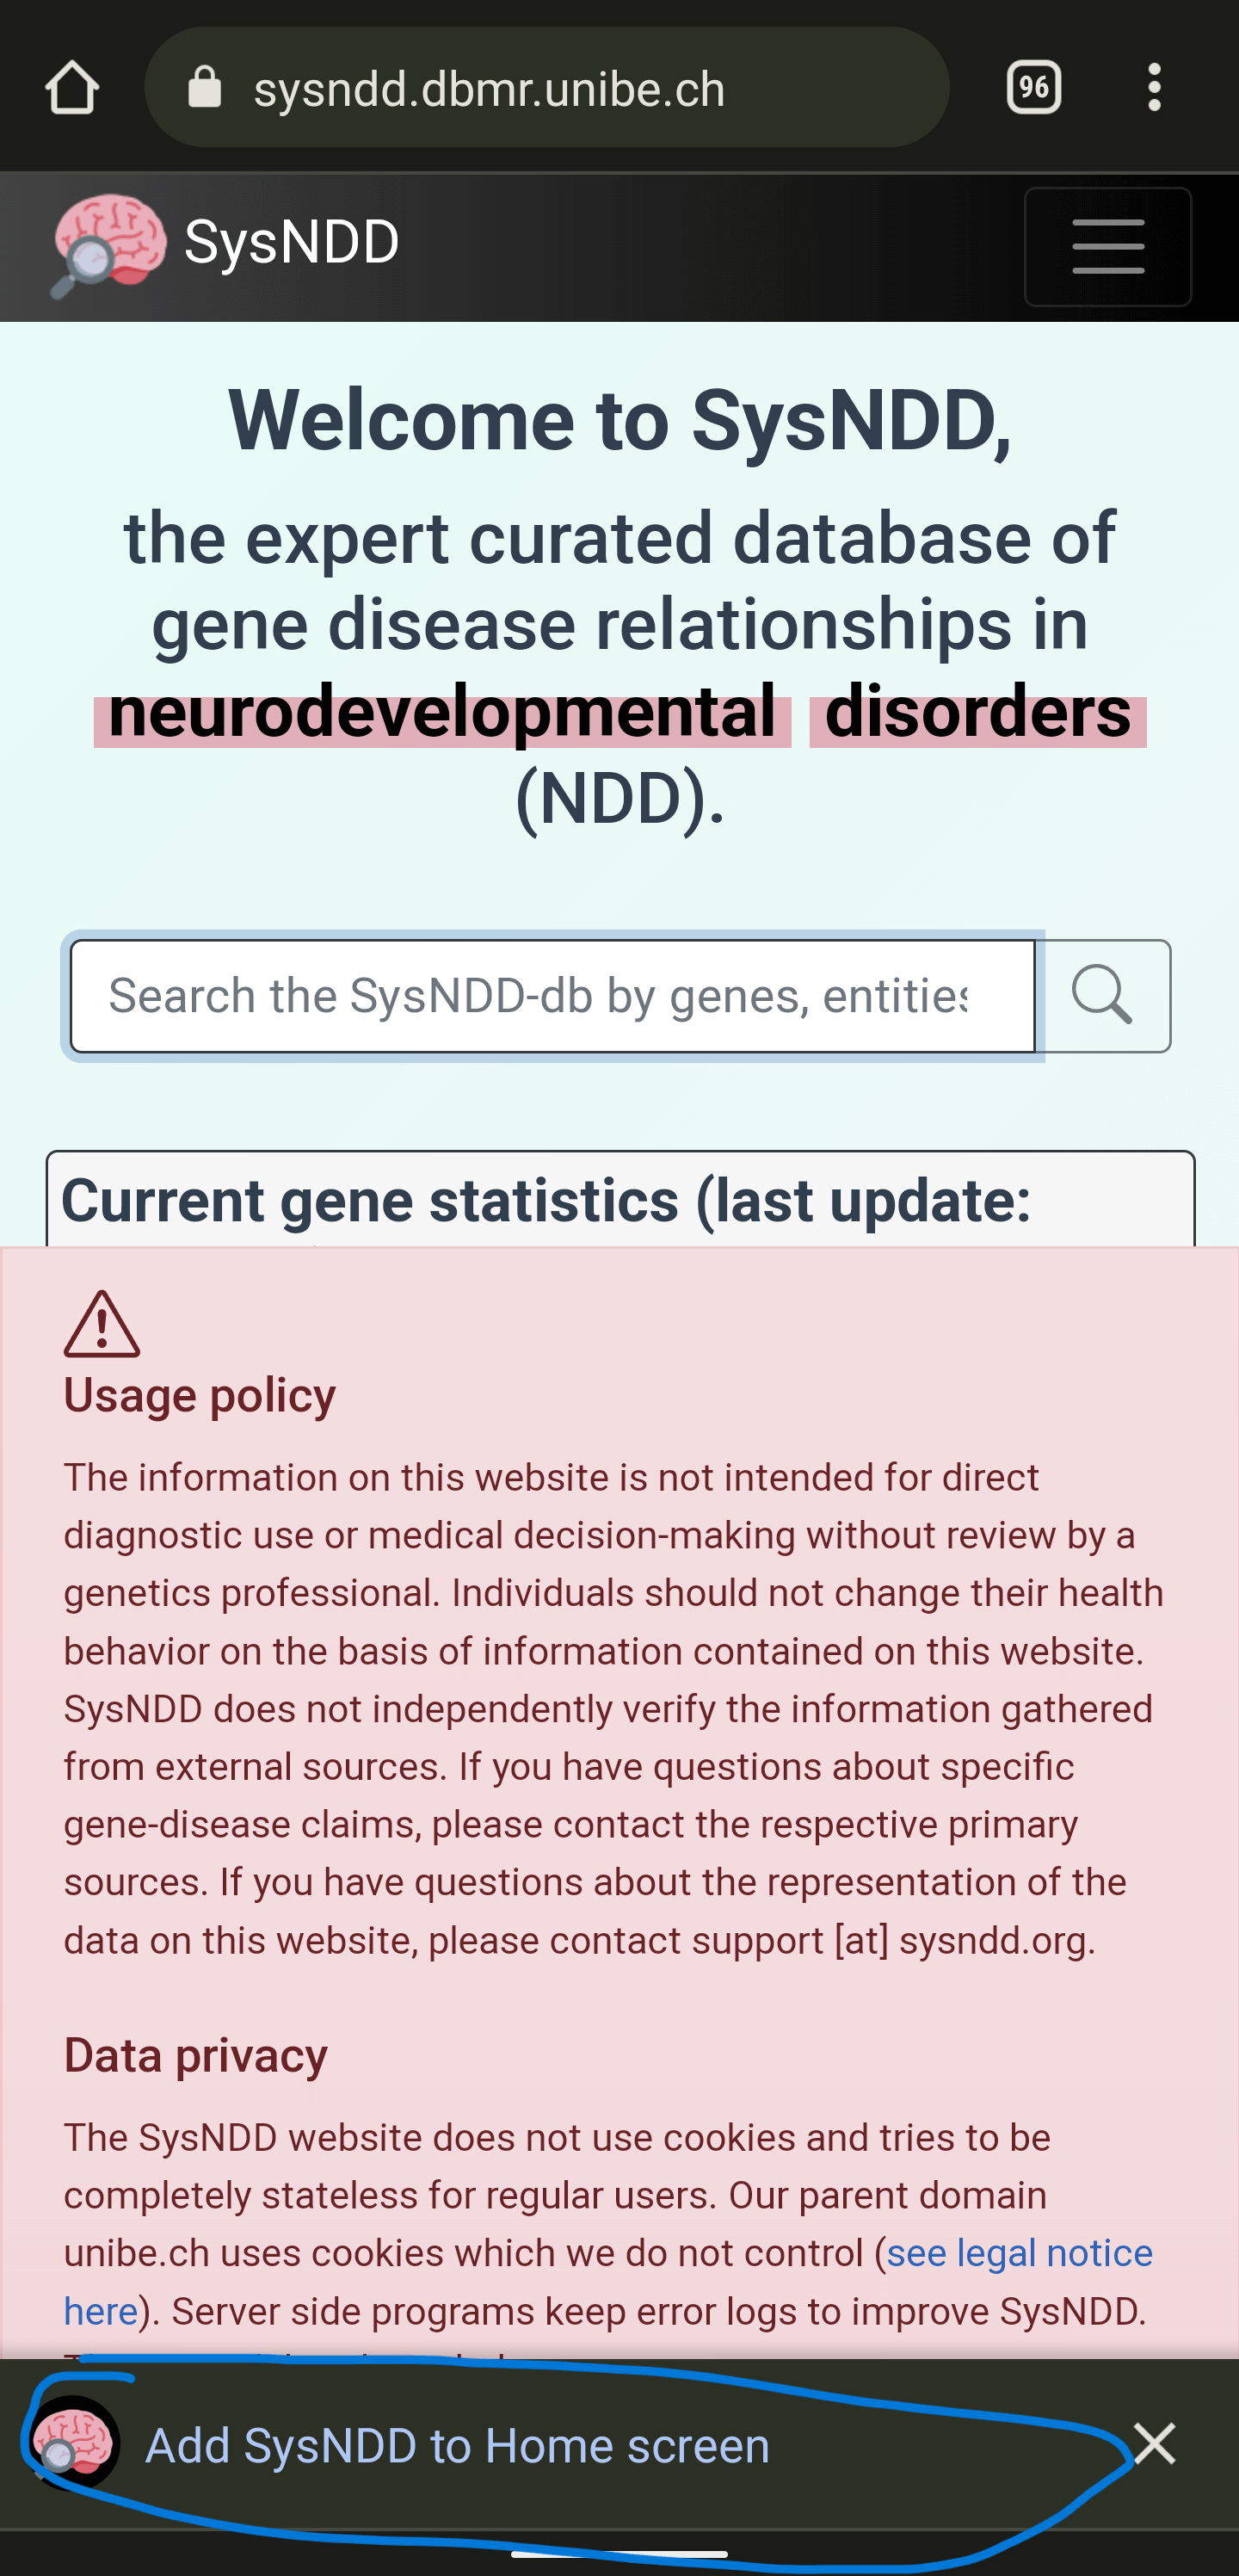
\includegraphics{./static/img/02_24-PWA-install-a.png}
\caption{PWA add}
\end{figure}

\textbf{2)} After clicking the previous message, confirm the installation by clicking ``Install'' in the following prompt:

\begin{figure}
\centering
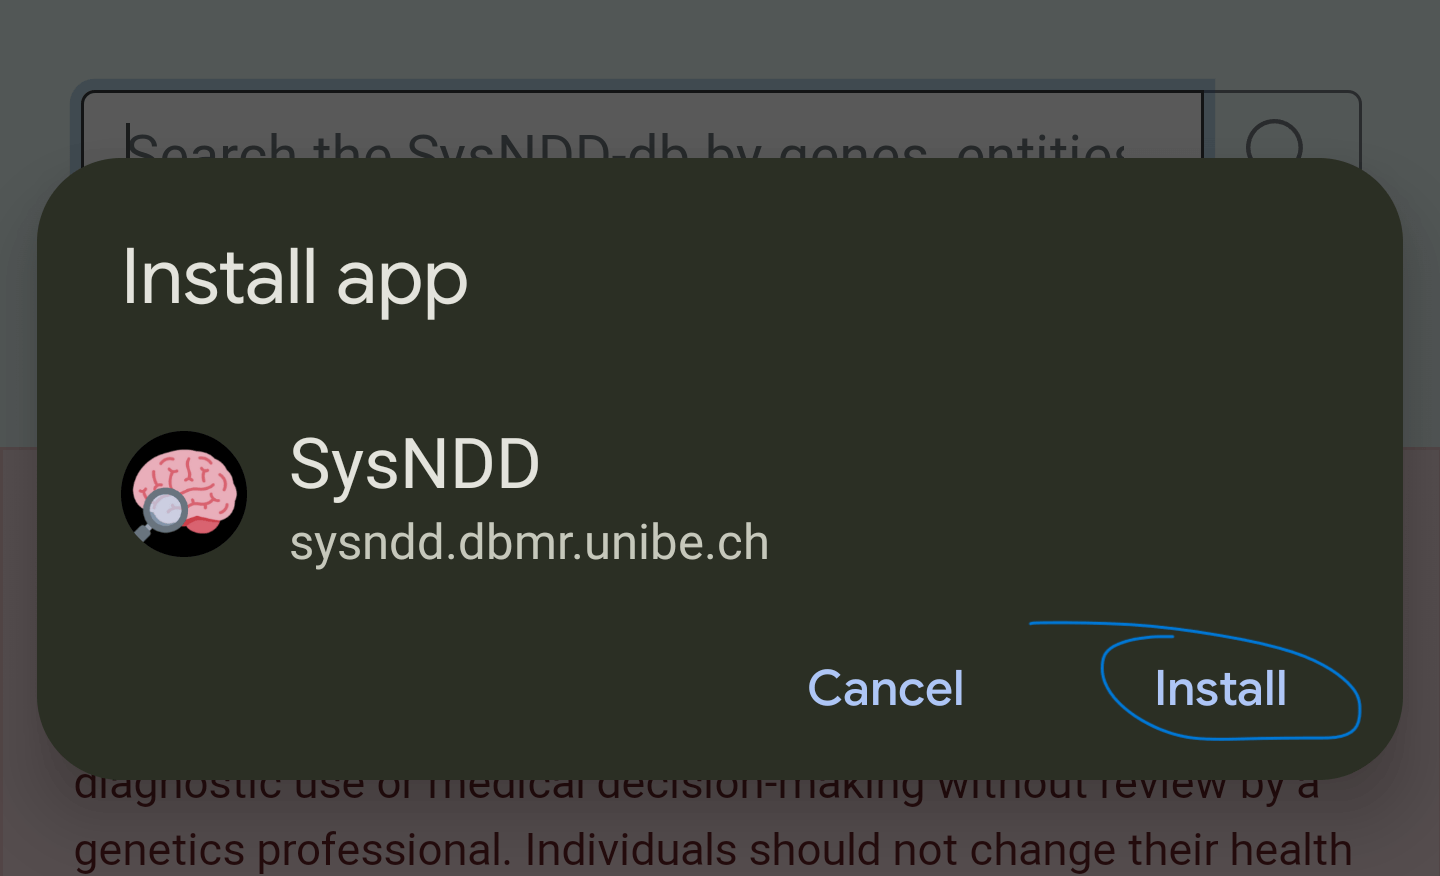
\includegraphics{./static/img/02_25-PWA-install-b.png}
\caption{PWA install}
\end{figure}

\textbf{3)} A message will confirm the installation:

\begin{figure}
\centering
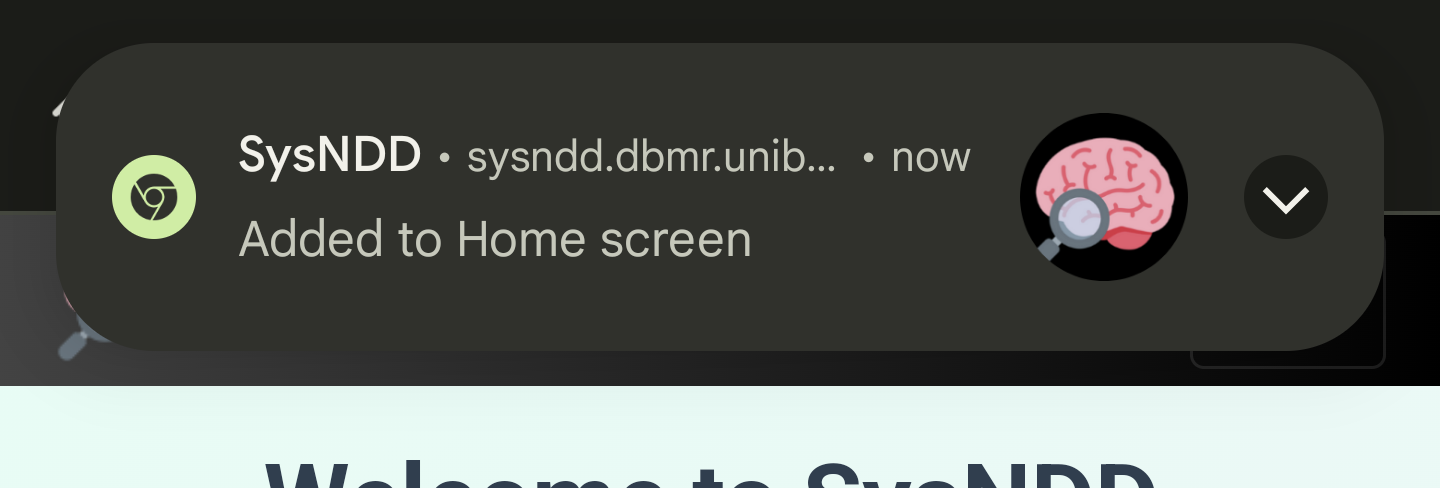
\includegraphics{./static/img/02_26-PWA-install-c.png}
\caption{PWA added}
\end{figure}

\textbf{4)} Following app symbol will be available on one of your screens:

\begin{figure}
\centering

\includegraphics{./static/img/02_27-PWA-install-d.png}
\caption{App symbol}
\end{figure}

\textbf{5)} Clicking this will open SysNDD in PWA mode (no browser adress bar, instead custom colored top bar):

\begin{figure}
\centering
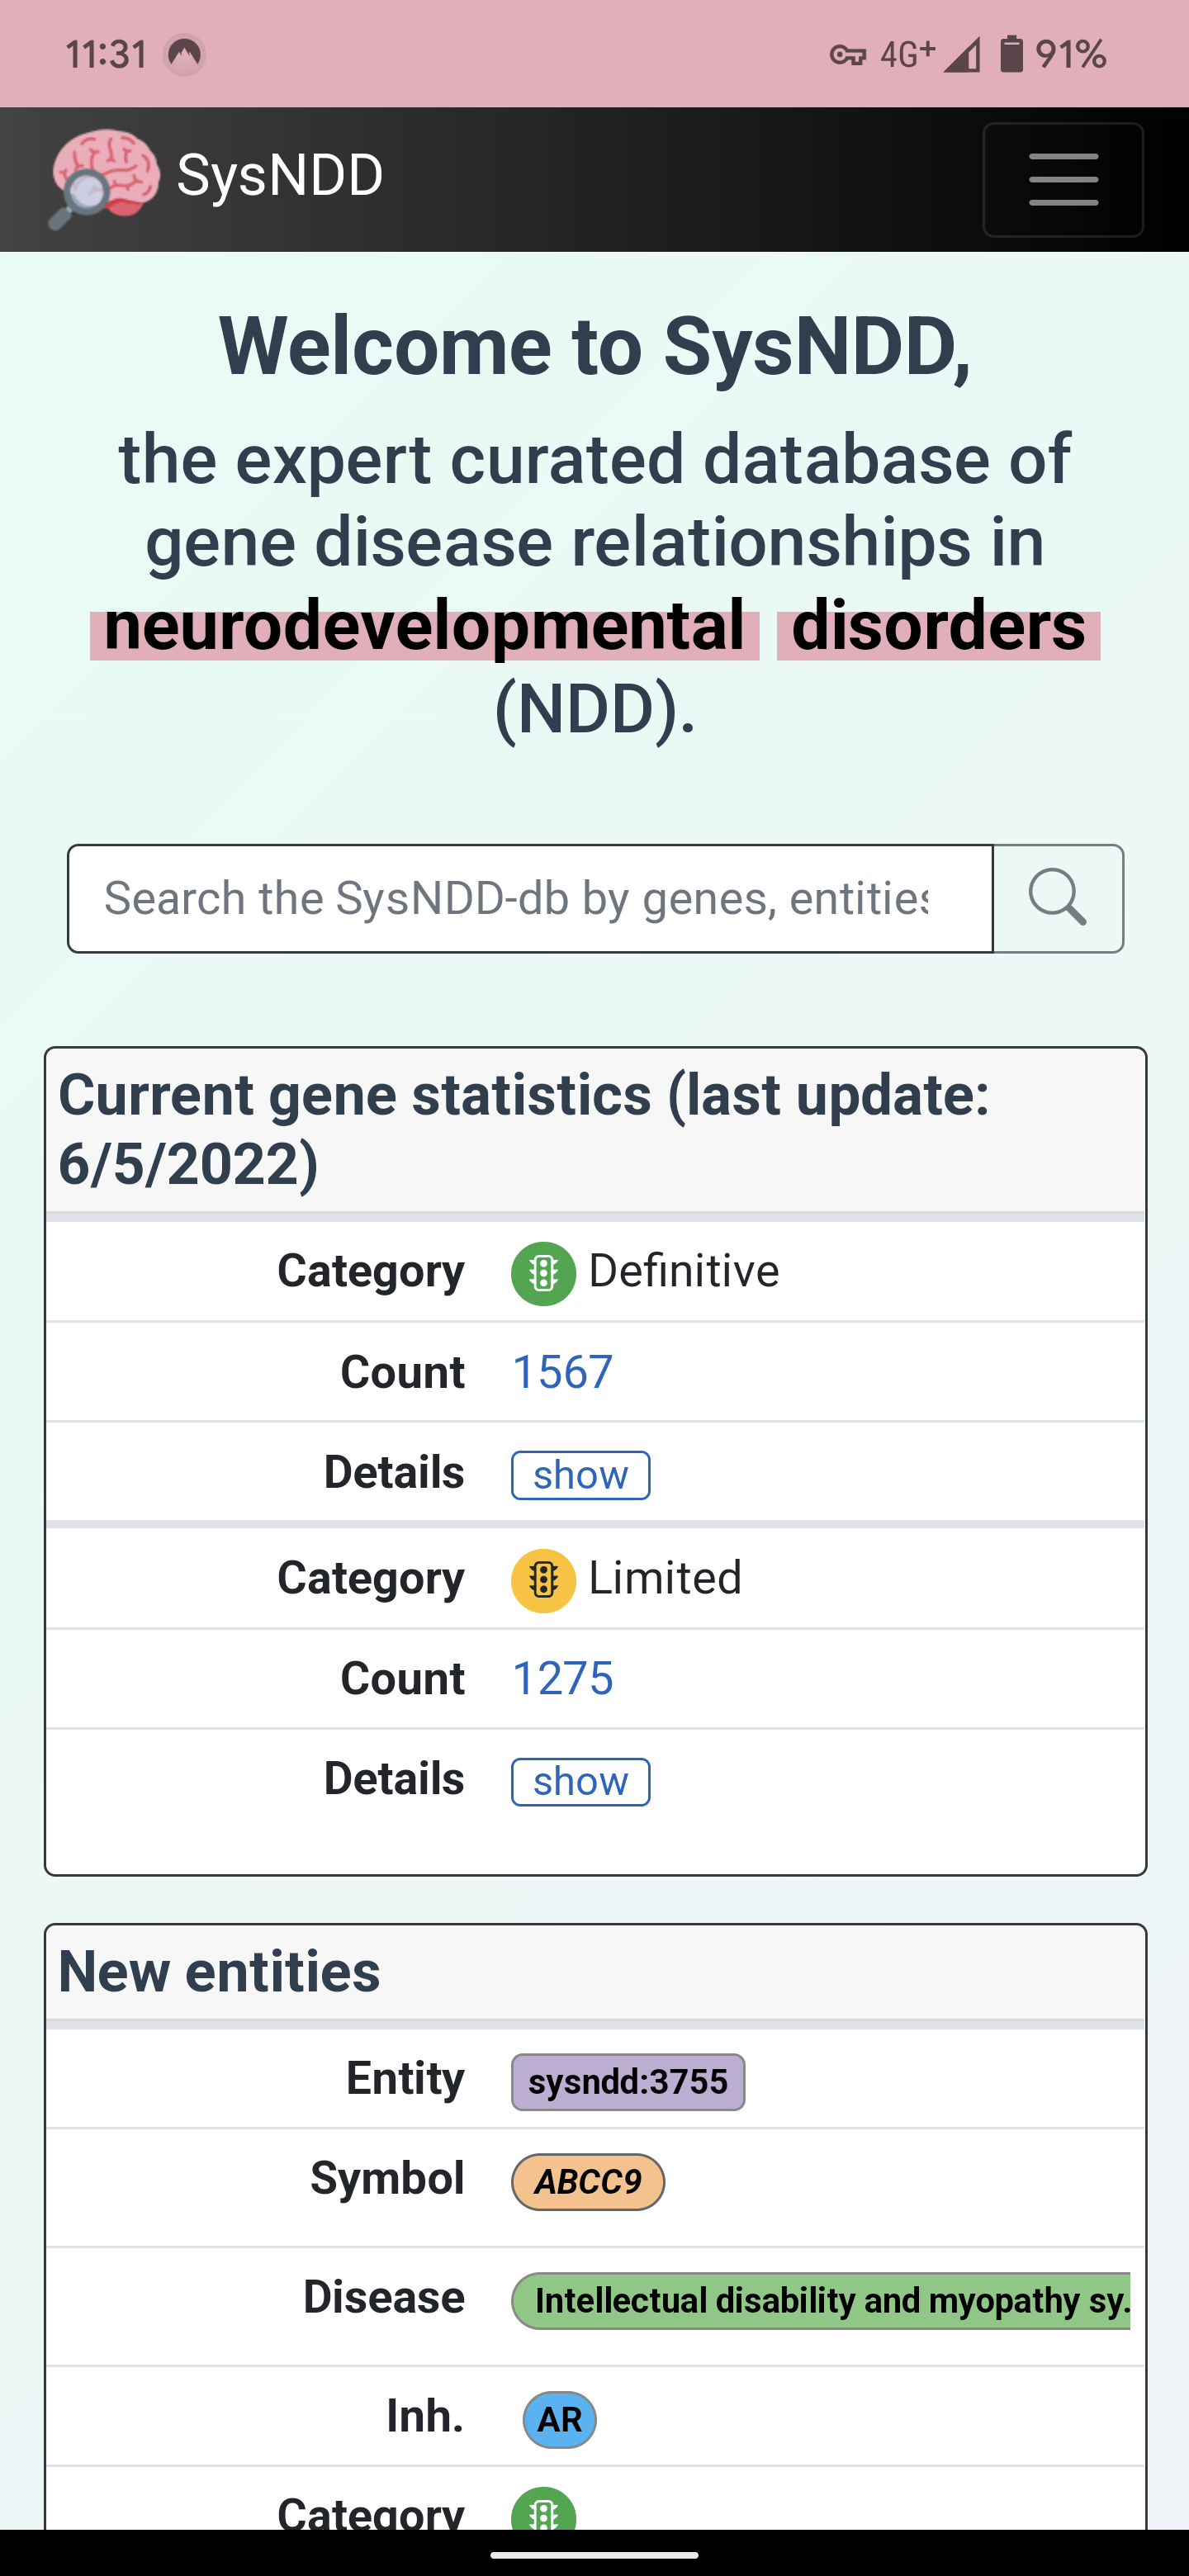
\includegraphics{./static/img/02_28-PWA-install-e.png}
\caption{PWA screenshot}
\end{figure}

\hypertarget{performance}{%
\subsection{Performance}\label{performance}}

Modern Javascript frameworks like Vue.js, which we use for the SysNDD website, offer rich user experience. The generated single-page applications can be slower then server side rendered pages.

With SysNDD we are engaged to provide a fast user experience by reducing component and request sizes and applying techniques like lazy loading and code splitting in the frontend with parallelisation in the api.

A quick overview on the current website performance can be obtained on PageSpeed Insights (or ``Lighthouse'' in the chrome development console):

\href{https://pagespeed.web.dev/report?url=https\%3A\%2F\%2Fsysndd.dbmr.unibe.ch\%2F\&form_factor=desktop}{https://pagespeed.web.dev/report?url=https\%3A\%2F\%2Fsysndd.dbmr.unibe.ch\%2F}

\hypertarget{security}{%
\subsection{Security}\label{security}}

SysNDD is engaged to offer highest security standards for all web tools.
We use HTTPS with Transport Layer Security (TLS) and follow the mozilla recommendations for web server settings.

A quick overview for our security settings for the SysNDD website can be obtained on Mozilla Oservatory:

\url{https://observatory.mozilla.org/analyze/sysndd.dbmr.unibe.ch}

\hypertarget{api}{%
\section{API}\label{api}}

\begin{center}\rule{0.5\linewidth}{0.5pt}\end{center}

The SysNDD api (application programming interface) is available from \url{https://sysndd.dbmr.unibe.ch/API}.

The api is written in R using the \href{https://www.rplumber.io/}{plumber package}.

We intend to follow the \href{https://swagger.io/specification/}{Swagger/ OpenAPI} and \href{https://jsonapi.org/}{JSON:API} specifications.

The api scripts run in a Docker container using the official ``rocker/tidyverse'' image (version 4.2.0).

As R is single threaded, we deploy multiple instances of the api container. These are bundled together using \href{http://www.haproxy.org/}{HAProxy} load balancer.

The api is rate limited through our \href{https://www.nginx.com/}{NGINX} web server configuration with a rate limit of 10 requests per second (10r/s; equals 1 request every 100 milliseconds) per requesting ip. The configuration allows bursts of up to 30r/s but introduces a delay after 10 requests to enforce the rate limit.

\hypertarget{endpoints}{%
\subsubsection{Endpoints}\label{endpoints}}

The SysNDD api currently contains all endpoints for externala nd internal usage in one api script. This may change with future releases.

The api is structured into different components based on the SysND concept:

\begin{itemize}
\tightlist
\item
  entity: Entity related endpoints
\item
  review: Reviews related endpoints
\item
  status: Status related endpoints
\item
  re\_review: Re-review related endpoints
\item
  publication: Publication related endpoints
\item
  gene: Gene related endpoints
\item
  ontology: Ontology related endpoints
\item
  inheritance: Inheritance related endpoints
\item
  phenotype: Phenoptype related endpoints
\item
  panels: Gene panel related endpoints
\item
  comparisons: NDD gene list comparisons related endpoints
\item
  search: Database search related endpoints
\item
  list: Database list related endpoints
\item
  statistics: Database statistics
\item
  user: User account related endpoints
\item
  authentication: Authentication related endpoints
\end{itemize}

The endpoints are documented and can be tested using the Swagger/ OpenAPI user interface at \url{https://sysndd.dbmr.unibe.ch/API}.
Here one can generate cURL requests to use in external software.

\hypertarget{usage-policy}{%
\subsubsection{Usage policy}\label{usage-policy}}

The SysNDD api powers the web tool for everyday users. We also provide the SysNDD api free to allow users to use the SysNDD data and build on it by creating software or services that connect to our platform.

Usage requirements:
- optimize your requests to stay in the above described limits
- be sensible about re-using data (e.g., store your requests until data is updated on our server)
- use pagination where possible instead of requesting large data chunks (e.g., restrict usage of ``all'' option in large, potentially blocking list endpoints like ``entity'' and ``gene'')
- if you require more api ressources please get in contact

Updates and disclaimer:
- We provide the SysNDD api as-is.
- Due to the current development status (version 0.X.Y) we may update or modify the api any time. These changes may affect your use of the api or the way your integration interacts with the api.

\hypertarget{authentication-and-authorization}{%
\subsubsection{Authentication and authorization}\label{authentication-and-authorization}}

The SysNDD api uses JSON Web Tokens (\href{https://jwt.io/}{JWT}) to implement stateless authentication and authorization.

The api user can manually (test purposes) request a token by entering their login credentials in the ionput form provided at the ``api/auth/authenticate'' endpoint:

\begin{figure}
\centering
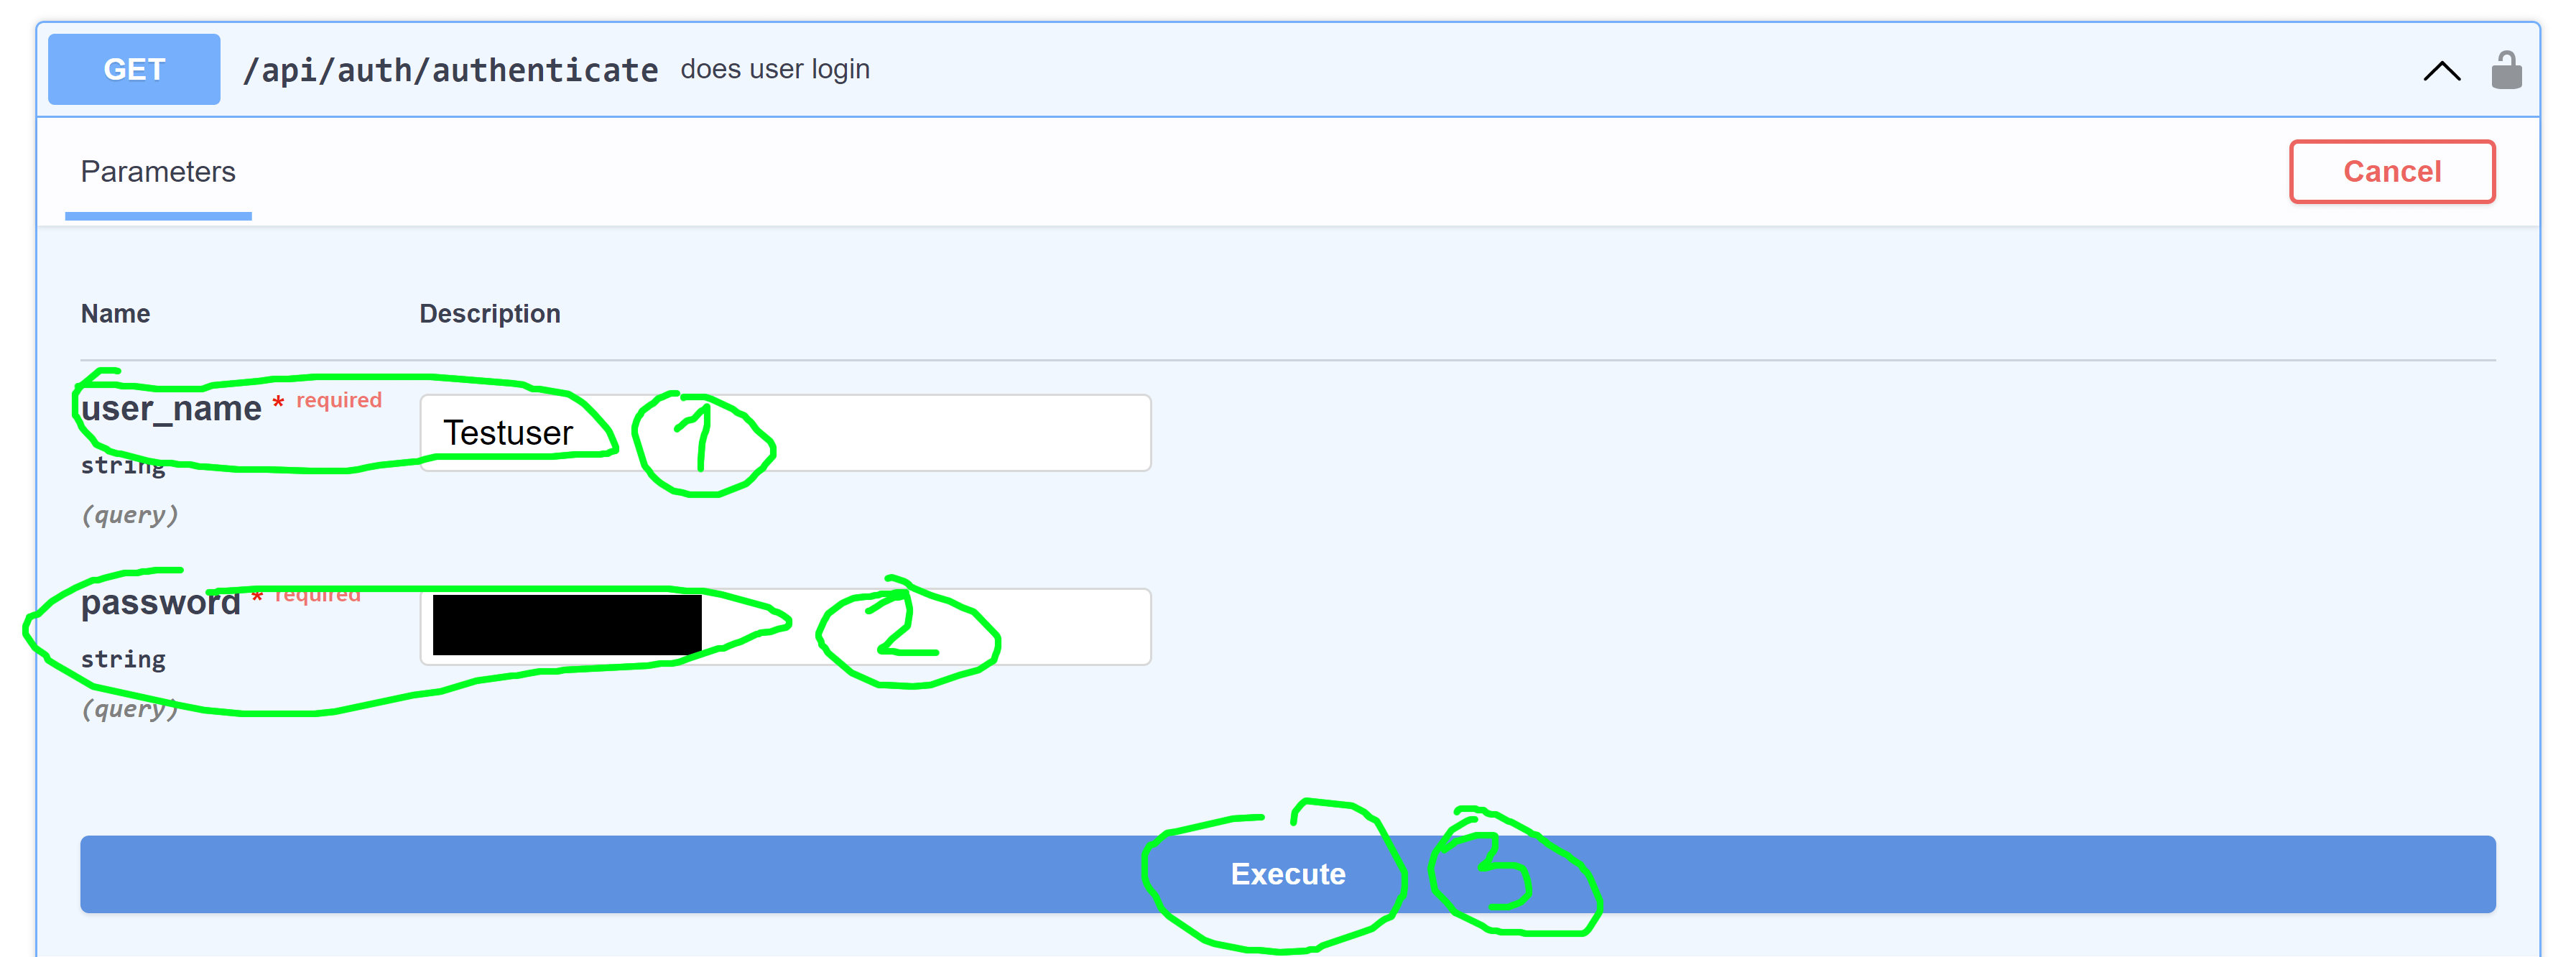
\includegraphics{./static/img/03_01-api-authenticate.png}
\caption{Authenticate endpoint}
\end{figure}

This endpoint will generate and respond with and JWT token:

\begin{figure}
\centering
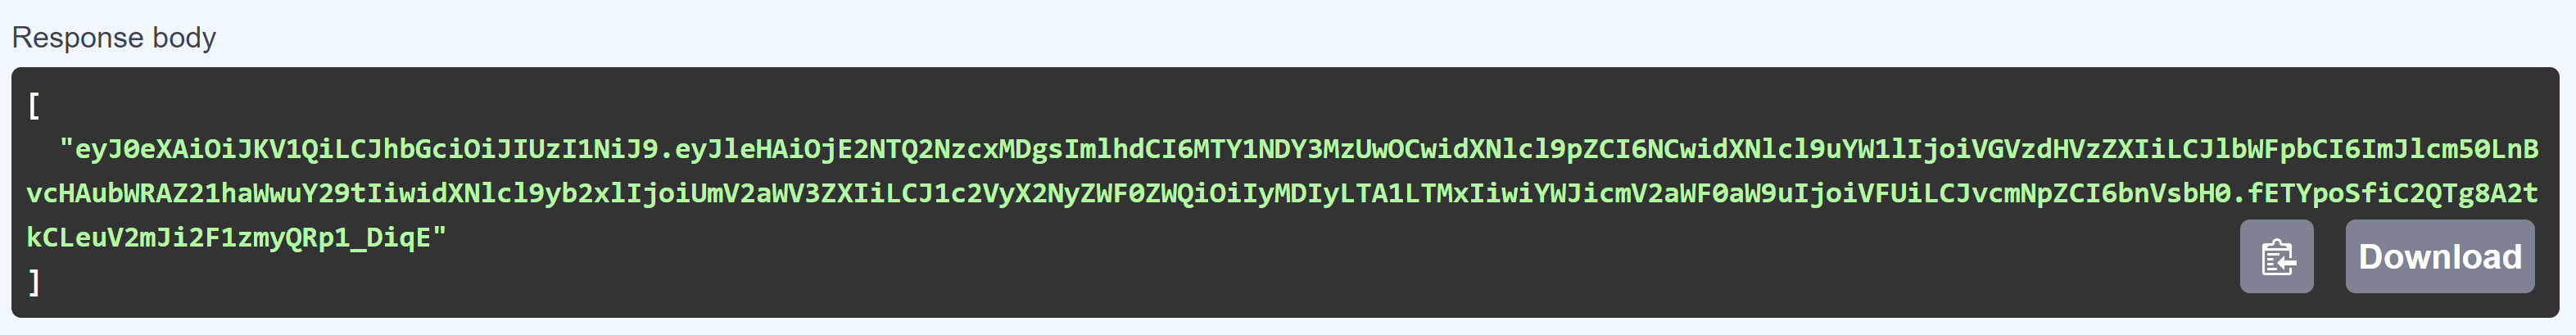
\includegraphics{./static/img/03_02-JWT-token.png}
\caption{JWT token}
\end{figure}

This Bearer token can then be copied and entered in the OpenAPI/ Swagger authorize modal which opens after clicking the ``Authorize'' modal button at the upper right corner:

\begin{figure}
\centering
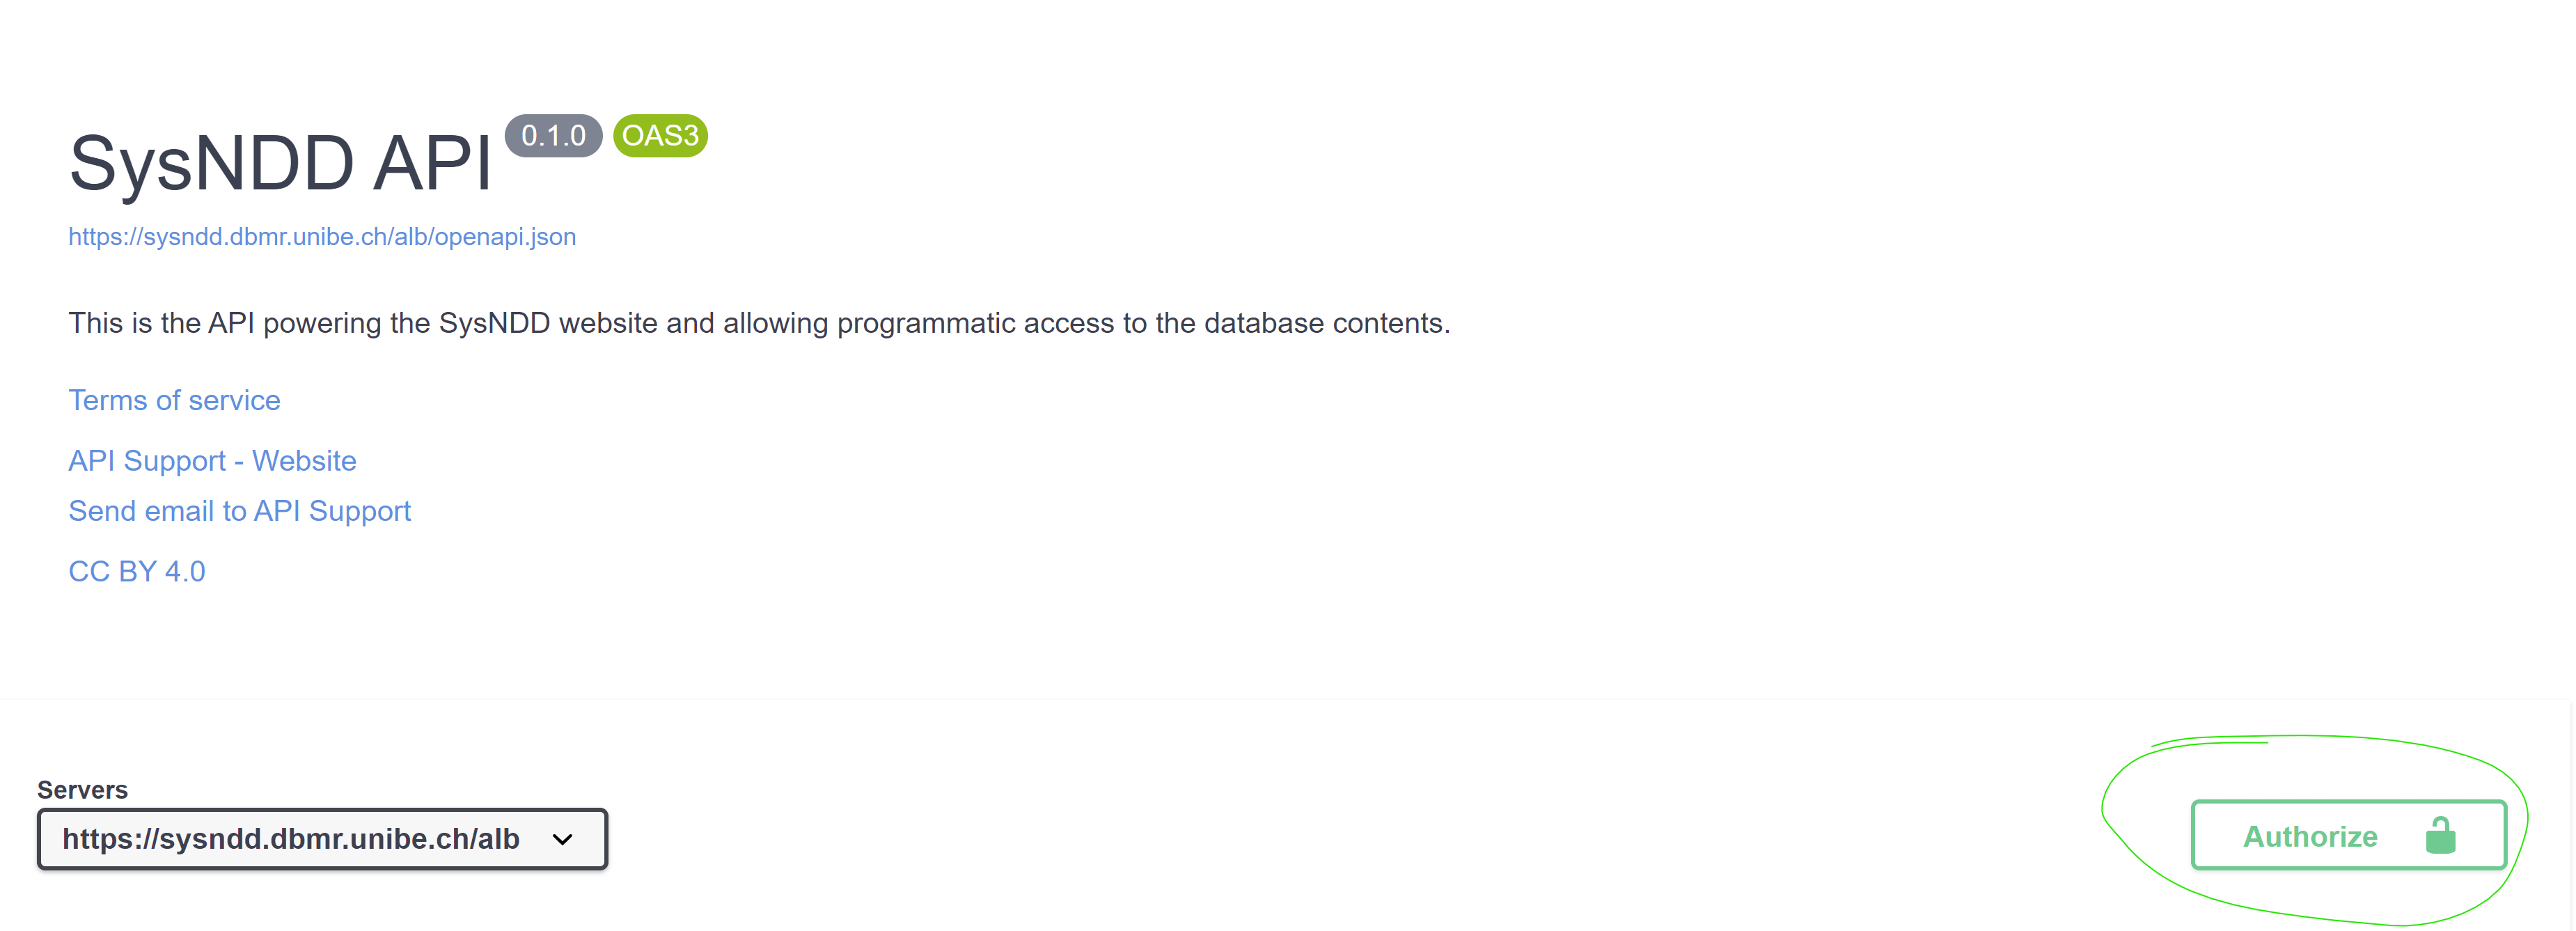
\includegraphics{./static/img/03_03-api-authorize-a.png}
\caption{Authorize button}
\end{figure}

\begin{figure}
\centering
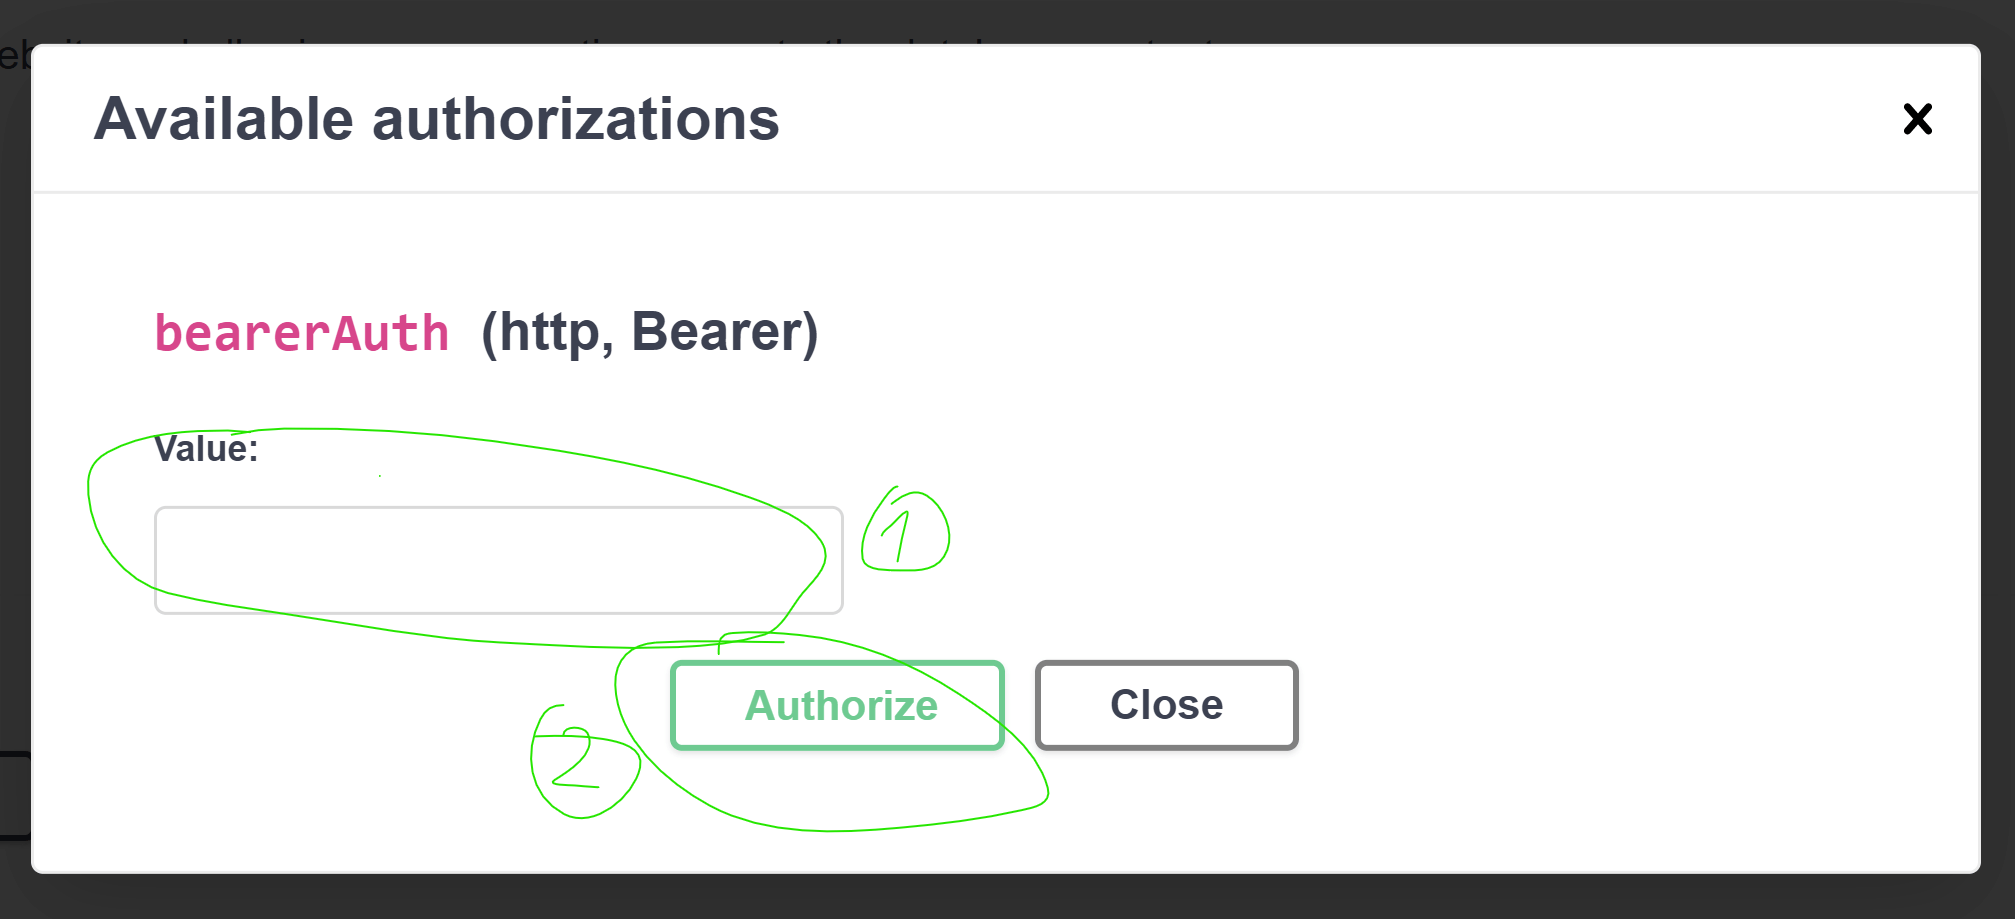
\includegraphics{./static/img/03_04-api-authorize-b.png}
\caption{Authorize modal prompt}
\end{figure}

After entereing the token in the respective field (1) and cklicking the ``Authorize'' submission button the modal will change and show the login status. This field can be closed now:

\begin{figure}
\centering
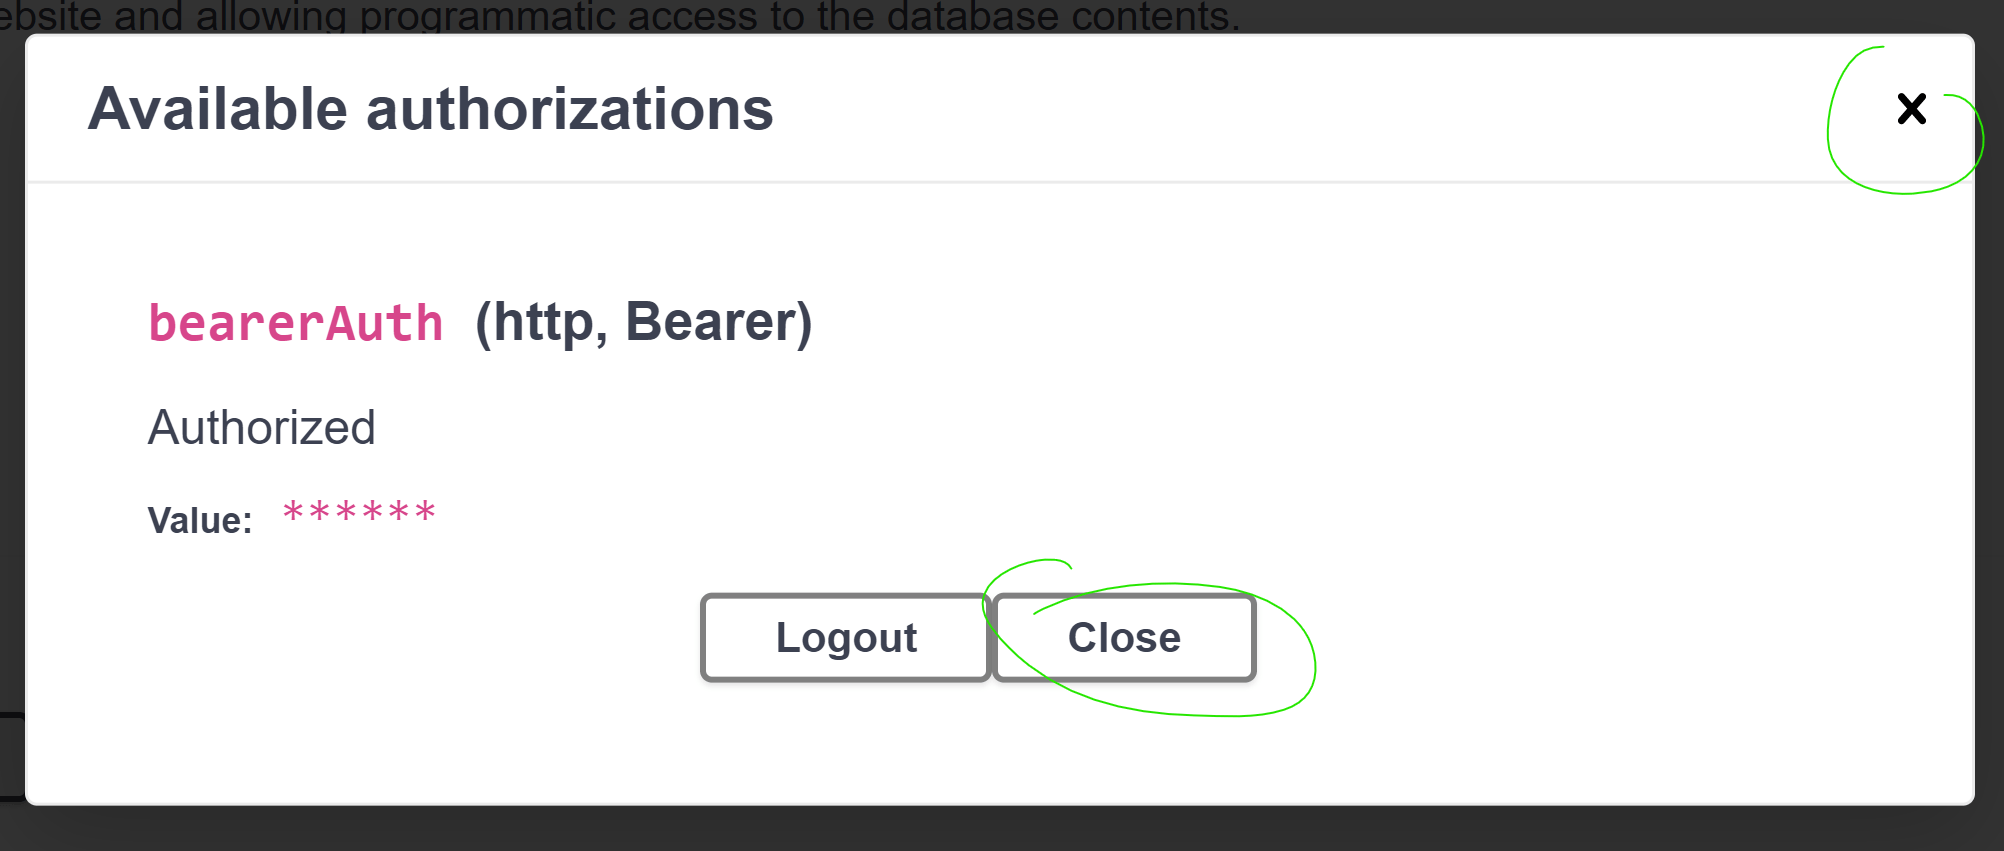
\includegraphics{./static/img/03_05-api-authorize-c.png}
\caption{Authorize modal logged in}
\end{figure}

The user is now fully authenticated and can access the endpoints requiring user rights:

\begin{figure}
\centering
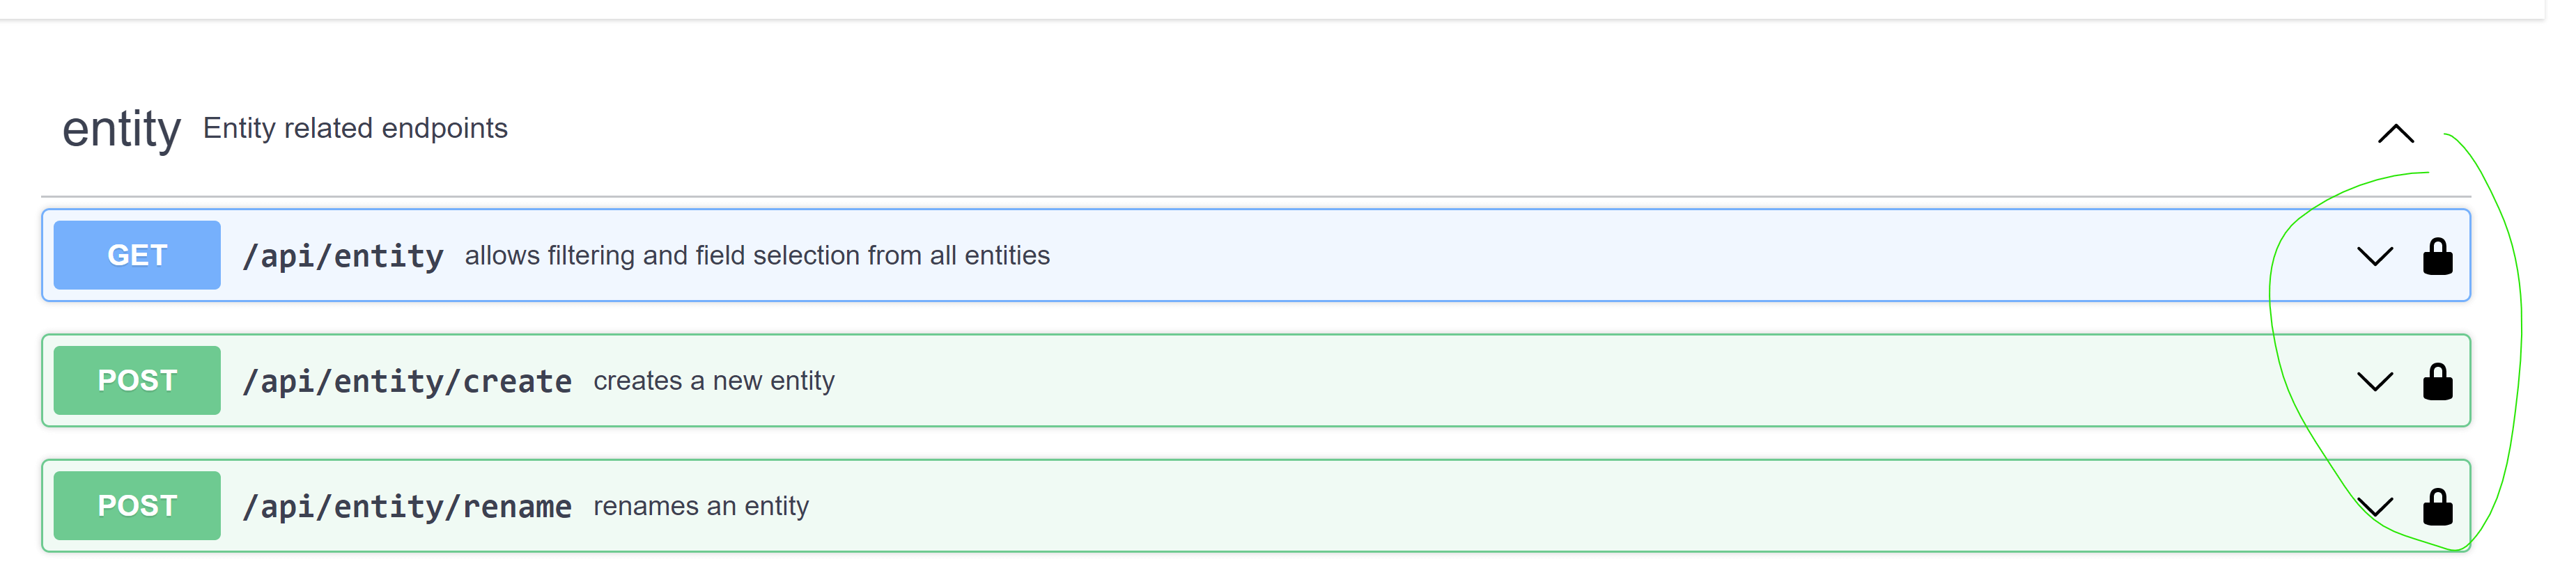
\includegraphics{./static/img/03_06-api-authorize-d.png}
\caption{API logged in}
\end{figure}

The token is valid for 60 minutes. It can be refreshed using the endpoint ``api/auth/refresh''.

\hypertarget{database-structure}{%
\section{Database structure}\label{database-structure}}

\begin{center}\rule{0.5\linewidth}{0.5pt}\end{center}

SysNDD currently uses the open-source \href{https://dev.mysql.com/doc/relnotes/mysql/8.0/en/}{MySQL 8.0} relational database management system (RDBMS).

The design of our DB schema can be viewed in \href{https://www.dbdesigner.net/}{DB DESIGNER}:

\href{https://dbdesigner.page.link/3Morx9HZxzqt4R379}{SysNDD DB schema}

As of 2022-06-07 the database schema looks like this:

\begin{figure}
\centering
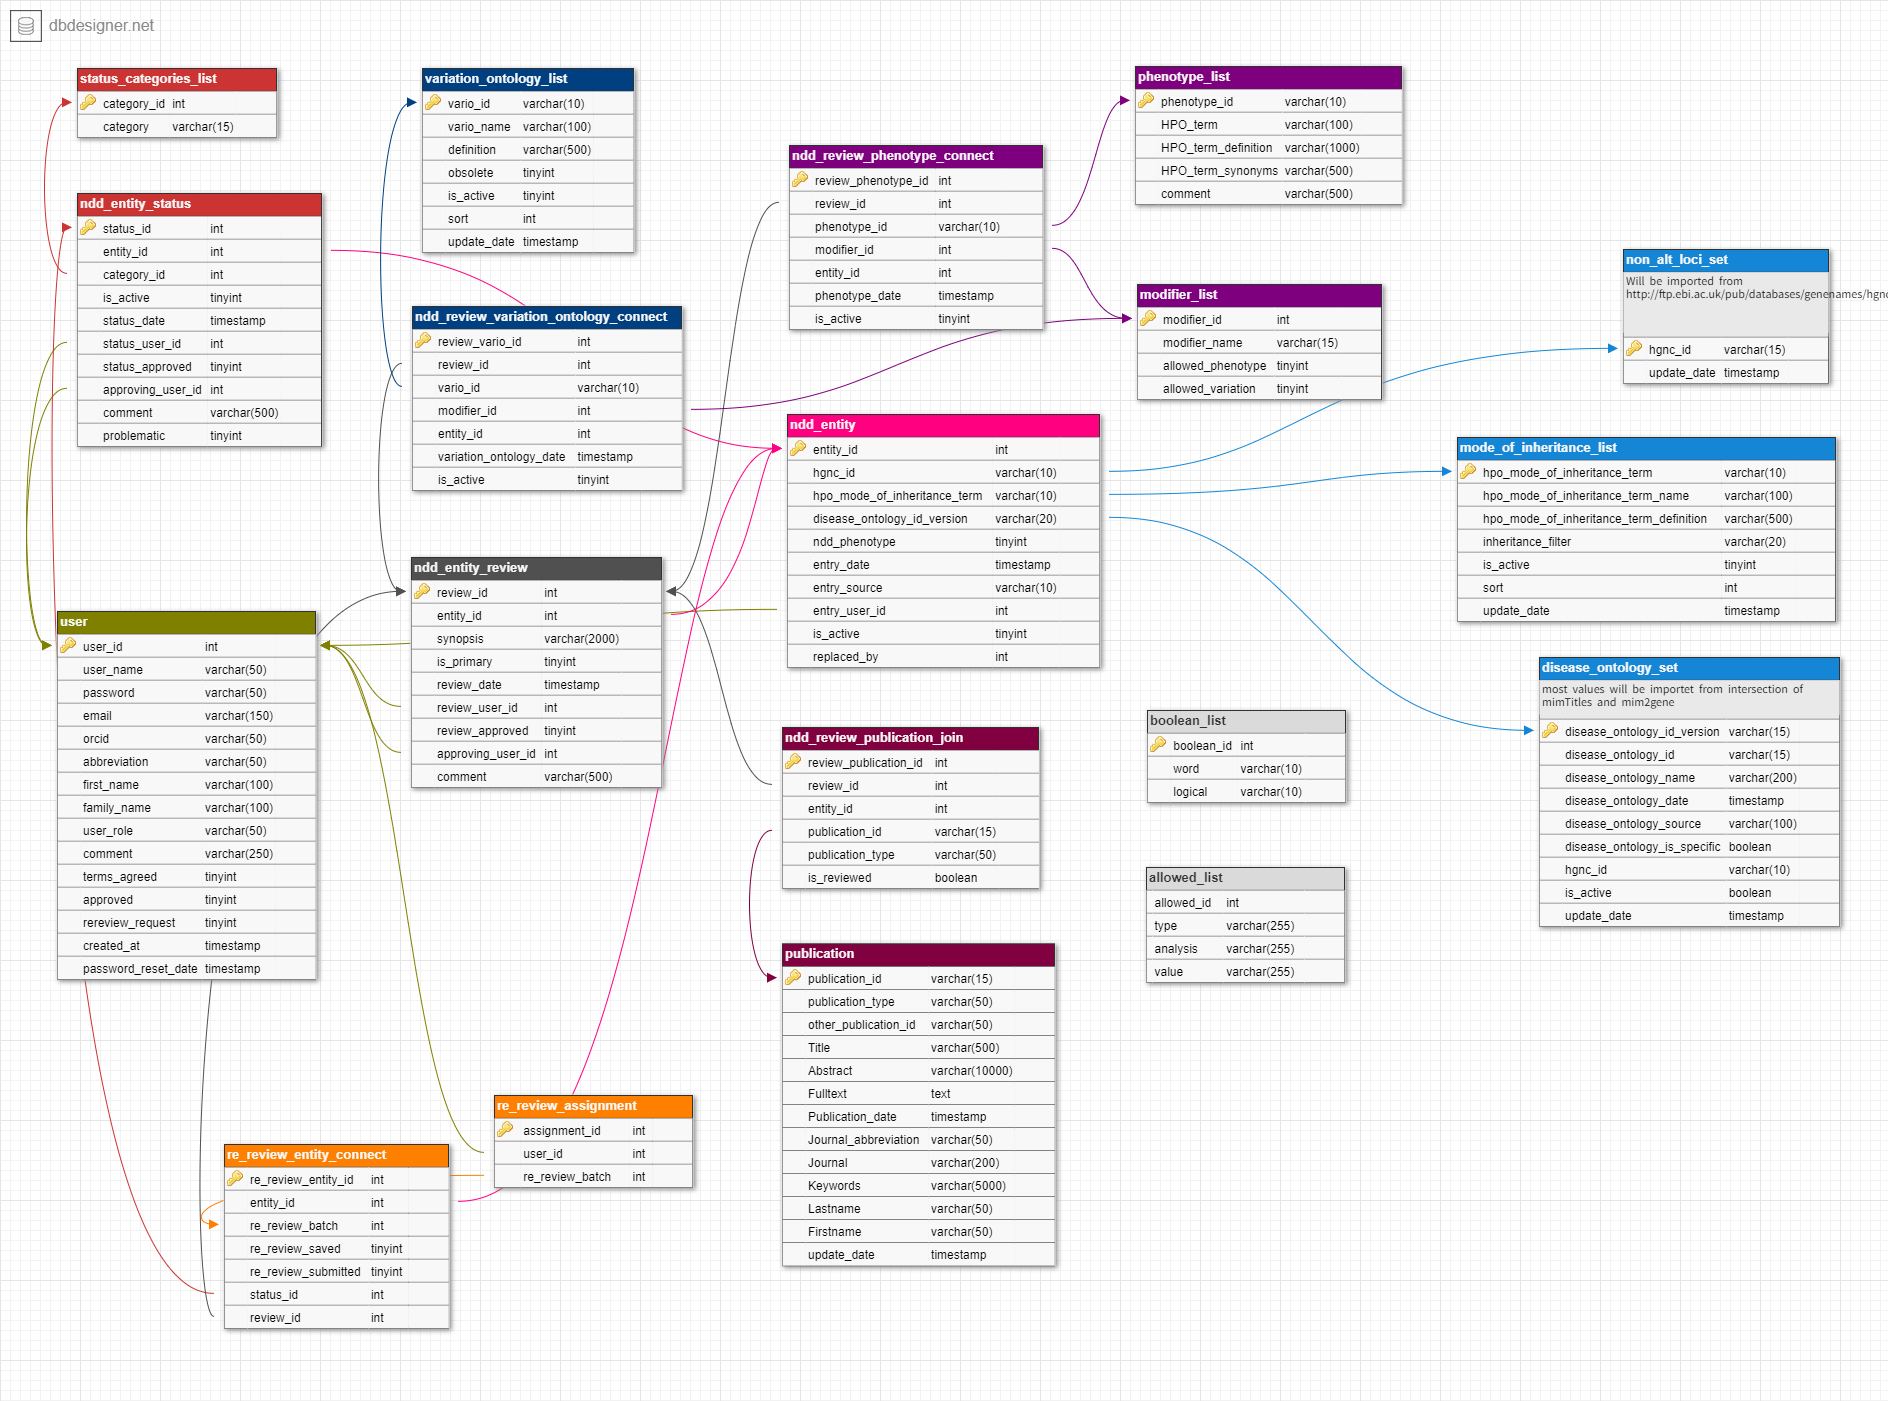
\includegraphics{./static/img/04_01-design-db-schema.png}
\caption{SysNDD MysQL database}
\end{figure}

The databse runs in a docker container using the \href{https://hub.docker.com/_/mysql}{official mysql docker image} (version 8.0.29).

\hypertarget{curation-criteria}{%
\section{Curation criteria}\label{curation-criteria}}

\begin{center}\rule{0.5\linewidth}{0.5pt}\end{center}

\hypertarget{definitions}{%
\subsection{Definitions}\label{definitions}}

Intellectual disability (ID) and neurodevelopmental disorders (NDD) are defined in the scope of SysNDD as follows:

\begin{itemize}
\tightlist
\item
  Early onset neurodevelopmental delay and cognitive impairment (severe ID to learning difficulties)
\item
  Regression/ neurodegeneration in the first years of life with or without prior developmental delay
\item
  Disorders with cognitive impairment in a significant (ca. \textgreater10\%) fraction of individuals
\end{itemize}

\hypertarget{ndd-definitive-entities}{%
\subsection{NDD Definitive entities}\label{ndd-definitive-entities}}

Inclusion criteria for Category 1 (``Definitive''):

\textbf{1.} Publication required (no grey literature like conference abstracts or personal communication; manuscripts on preprint servers can be considered individually but only entered through their DOI in the comment field until published with PMID, when they should be updated)

\textbf{AND}

\textbf{2.} Clear-cut frequency (no further criteria needed)

\begin{itemize}
\tightlist
\item
  \textgreater= 10 cases with \emph{de novo} variants
\item
  \textgreater= 5 autosomal-recessive families
\item
  \textgreater= 3 families with X-chromosomal variants
\end{itemize}

\textbf{OR}

\textbf{3.} Cumulative evidence

\begin{itemize}
\tightlist
\item
  1 strong frequency criterium
\end{itemize}

\textbf{PLUS}

\begin{itemize}
\tightlist
\item
  1 strong genetic or 1 strong clinical criterium
\end{itemize}

\textbf{OR}

\begin{itemize}
\tightlist
\item
  2 further strong (genetic and/or clinical) criteria in case of only 2 families with recessive inheritance
\end{itemize}

\textbf{OR}

\begin{itemize}
\tightlist
\item
  \textgreater= two moderate criteria
\end{itemize}

\hypertarget{strong-criteria}{%
\subsubsection{Strong criteria}\label{strong-criteria}}

Strong frequency criteria:

\begin{itemize}
\tightlist
\item
  \textgreater= 3 patients with \emph{de novo} variant
\item
  \textgreater= 2 families with bi-allelic truncating variants
\item
  \textgreater= (2-)3 families with bi-allelic missense variants
\item
  \textgreater= 2 families with X-chromosomal variants
\end{itemize}

Strong genetic criteria:

\begin{itemize}
\tightlist
\item
  recurrence of a variant
\item
  clustering of variants
\item
  \emph{de novo} truncating variants in a gene intolerant to loss-of-function variants (gnomAD constraint score)
\end{itemize}

Strong clinical criteria:

\begin{itemize}
\tightlist
\item
  Homogeneous phenotype
\item
  Presence of specific/distinct clinical aspects (e.g., recognizable facial gestalt; rare specific malformations; pattern of multiple malformation; characteristic MRI anomalies; specific metabolic/enzymatic anomalies)
\end{itemize}

\hypertarget{moderate-criteria}{%
\subsubsection{Moderate criteria}\label{moderate-criteria}}

\begin{itemize}
\tightlist
\item
  Multigenerational segregation of variants
\item
  Functional tests
\item
  Gene involved in a pathway/complex where variants in other subunits are associated with a similar phenotype
\item
  \emph{De novo} missense variants in a gene intolerant to missense variants (gnomAD constraint scores)
\end{itemize}

\hypertarget{possible-negative-criteria}{%
\subsubsection{Possible negative criteria}\label{possible-negative-criteria}}

These should be included into consideration in borderline cases.

\begin{itemize}
\tightlist
\item
  Age of first publication(s) without further confirmatory reports in the meantime
\item
  Publication quality and journal or genetics expertise ``doubtful''
\item
  New evidence against gene and/or variants: e.g., constraint scores, frequencies in gnomAD
\end{itemize}

\hypertarget{ndd-moderate-and-limited-entities}{%
\subsection{NDD Moderate and Limited entities}\label{ndd-moderate-and-limited-entities}}

These categories include the previous category of ``candidate genes'' and are now split into criteria for entity categories 2 (``Moderate'') and 3 (``Limited''):

\textbf{1.} Must be published (no private, in-house candidate lists)

\textbf{AND}

\textbf{2.} ID indicated, but criteria not sufficient for category 1, examples:

\textbf{a.} Limited genetic evidence

\begin{itemize}
\tightlist
\item
  \textless{} 3 cases with \emph{de novo}, different variants and non-specific NDD phenotype
\item
  1 recessive family with truncating variant or \textless= 2 recessive families with missense variants (category 2 or 3 depending on number of affected and tested individuals per family, functional evidence and homogeneity of phenotype etc.)
\item
  candidate gene from translocation or larger deletion
\item
  reports of enzymatically confirmed patients with specific metabolic disorders but without genetic mutation confirmed
\end{itemize}

\textbf{b.} Limited clinical evidence

\begin{itemize}
\tightlist
\item
  not much evidence for ID, e.g.~reported as ADHD or ASD or neurological disorder without clearly reported low IQ and ID
\item
  known disorder, but only single patients reported with ID
\item
  motor developmental delay without evidence for cognitive impairment
\item
  clear neurodegenerative course without ID or cognitive delay present in the first years
\item
  lethal before ID might be evident, although e.g.~brain malformations or metabolic abnormalities might point to ID
\item
  ID reported in other, similar disorders caused by mutations in the same pathway/complex but not (yet) in association with this particular gene (e.g.~Fanconi anemia)
\end{itemize}

\textbf{c.} Limited combined genetic and clinical evidence

\begin{itemize}
\tightlist
\item
  Gene enriched for de novo or rare deleterious variants in large NDD cohorts or meta-studies, no further details
\end{itemize}

\hypertarget{exclusion-criteria}{%
\subsubsection{Exclusion criteria}\label{exclusion-criteria}}

\begin{enumerate}
\def\labelenumi{\arabic{enumi}.}
\tightlist
\item
  Published as candidate gene only based on function or experimental results but without variants reported in humans
\end{enumerate}

\textbf{AND/OR}

\begin{enumerate}
\def\labelenumi{\arabic{enumi}.}
\setcounter{enumi}{1}
\tightlist
\item
  Only 1 \emph{de novo} case from longer ago without further evidence and gene tolerant towards missense and/or loss-of-function variants according to gnomAD constraint scores
\end{enumerate}

\textbf{AND/OR}

\begin{enumerate}
\def\labelenumi{\arabic{enumi}.}
\setcounter{enumi}{2}
\tightlist
\item
  Only 1 sporadic case with bi-allelic variants and without any further supporting evidence such as segregation in other family members, functional tests, similar phenotypes in other patients with variants in genes from the same pathway, etc.
\end{enumerate}

\hypertarget{when-to-choose-category-2-moderate}{%
\subsubsection{When to choose category 2 (``Moderate'')?}\label{when-to-choose-category-2-moderate}}

Too good for category 3 (``Limited'') but not good enough for category 1 (``Definitive'')

Examples:

\begin{itemize}
\item
  Recurrent de novo variant in 2 individuals with a similar phenotype
\item
  Bi-allelic or X-chromosomal truncating variant segregating in \textgreater= two generations of a large family
\item
  Convincing functional evidence
\item
  1-2 patients with convincing variants in a gene which is in the same complex/pathway with other known disease genes and phenotype fits (e.g.~CDG syndrome)
\end{itemize}

\hypertarget{special-case-non-ndd-entities}{%
\subsubsection{Special case: non-NDD entities}\label{special-case-non-ndd-entities}}

Some genes are associated with multiple entities. Among these entities there might be some without ID as a clinical feature. These non-NDD entities will be included in SysNDD but they will not be classified to any of the categories. Instead, they are tagged with ``n.a.'' (not applicable).

\hypertarget{re-review-instructions}{%
\section{Re-review instructions}\label{re-review-instructions}}

\begin{center}\rule{0.5\linewidth}{0.5pt}\end{center}

The goal of the SysNDD ``Re-Review'' effort is to update and standardize the SysID entities collected during the past years to enable better integration into and interoperability international with gene curations.

\hypertarget{re-review-tool-usage}{%
\subsection{Re-review tool usage}\label{re-review-tool-usage}}

We created Reviewer status accounts for participating scientists.

\hypertarget{login}{%
\subsubsection{Login}\label{login}}

You can log into your account by pointing your browser to \url{https://sysndd.dbmr.unibe.ch/} and then clicking the ``Login`` link on the right side of the menu:

\begin{figure}
\centering
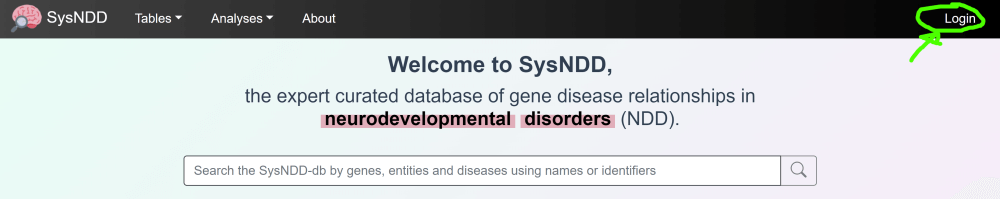
\includegraphics{./static/img/sysndd_login.png}
\caption{Login menu}
\end{figure}

On the Login page enter your credentials and press the Login button:

\begin{figure}
\centering
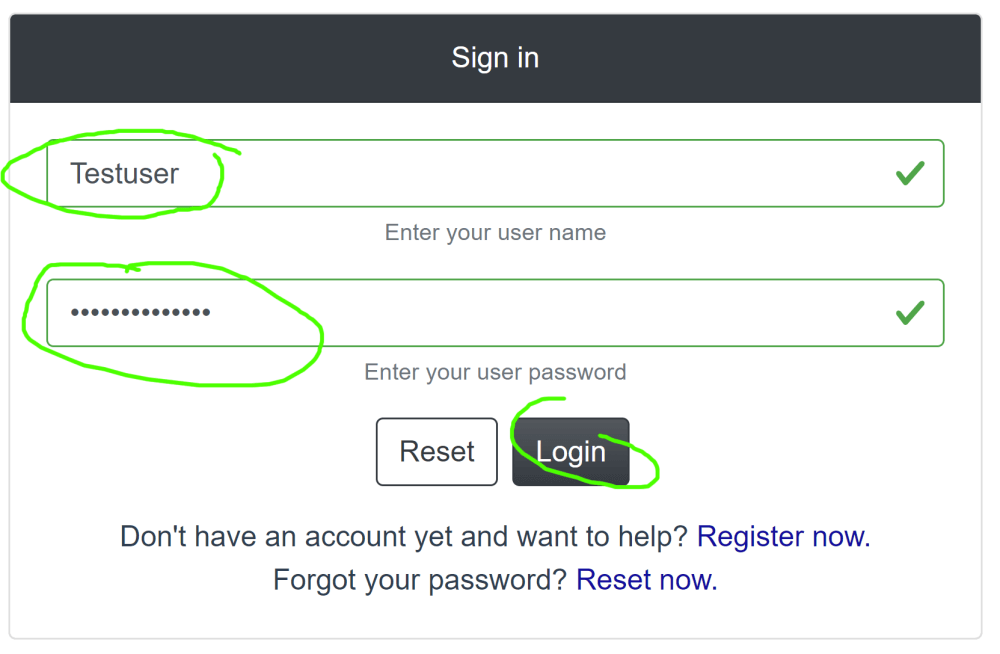
\includegraphics{./static/img/sysndd_login_page.png}
\caption{Login page}
\end{figure}

After successful login, you will be redirected to the start page and the navigation bar will show new links depending on your account privileges:

\begin{figure}
\centering
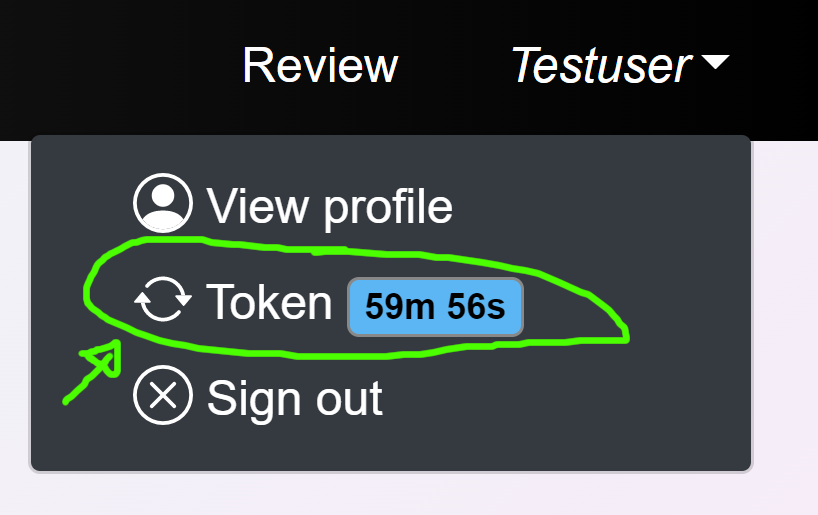
\includegraphics{./static/img/sysndd_refresh_token.png}
\caption{Login token menu}
\end{figure}

Your login token (JWT; JSON Web Token) is valid for 1 hour, after which you will be logged out. You can however always refresh the time by clicking the link in the user menu. The website will warn you at 5, 3 and 1 minutes before log out.

\hypertarget{review-page}{%
\subsubsection{Review page}\label{review-page}}

Click the ``Review'' link to your personal ``Re-Review'' site:

\begin{figure}
\centering
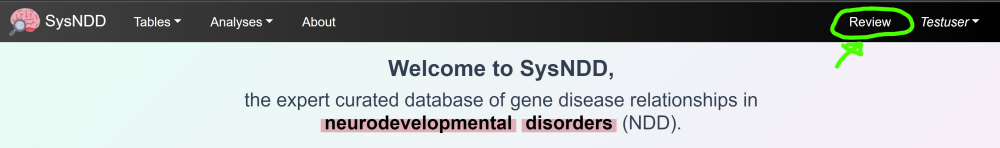
\includegraphics{./static/img/sysndd_review_page_menu.png}
\caption{Review page menu}
\end{figure}

The ``Re-Review'' page is structured as a table enriched with information and controls.

\begin{figure}
\centering
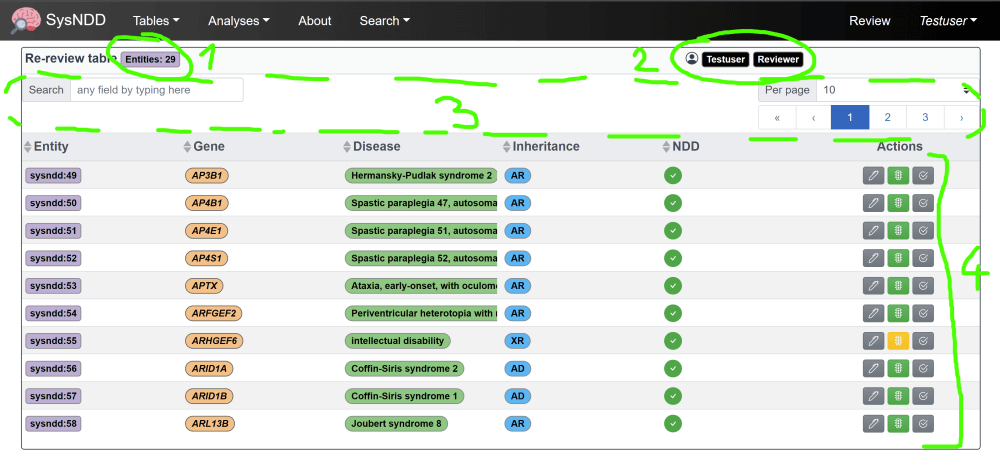
\includegraphics{./static/img/sysndd_review_page.png}
\caption{Review page}
\end{figure}

These show you the number of entities assigned to your account

~~~~ \textbf{(1)} your account information status specific controls (e.g.~switching to ``Curator'' mode, applying for a new batch of entities)

~~~~ \textbf{(2)} menu items to filter/ navigate the table

~~~~ \textbf{(3)} and finally, the table with the entity information and

~~~~ \textbf{(4)} controls to review and change the information:

By clicking the action buttons, you can open 3 different windows to change the entities review:

~~~~ \textbf{(1)} entities review (
\includegraphics{./static/img/edit_review_button.png})

~~~~ \textbf{(2)} the status (
\includegraphics{./static/img/edit_status_button.png})

~~~~ \textbf{(3)} and to submit your work (
\includegraphics{./static/img/submit_re-review_button.png})

\hypertarget{new-review-edit}{%
\subsubsection{New Review edit}\label{new-review-edit}}

In this window you have:

\begin{itemize}
\tightlist
\item
  the possibility to change/adapt or completely rewrite the current synopsis \textbf{(1)},
\item
  add, or remove phenotype associations \textbf{(2)},
\item
  add or remove publications from the review by PMID \textbf{(3)}
\item
  and add/ edit fitting GeneReviews articles by PMID \textbf{(4)}.
\item
  Finally, you can add a comment to your review for the Curator later approving this entities changes \textbf{(5)} and
\item
  save your review \textbf{(6)}.
\end{itemize}

By clicking on the little question marks you can show help messages for each item:

\begin{figure}
\centering
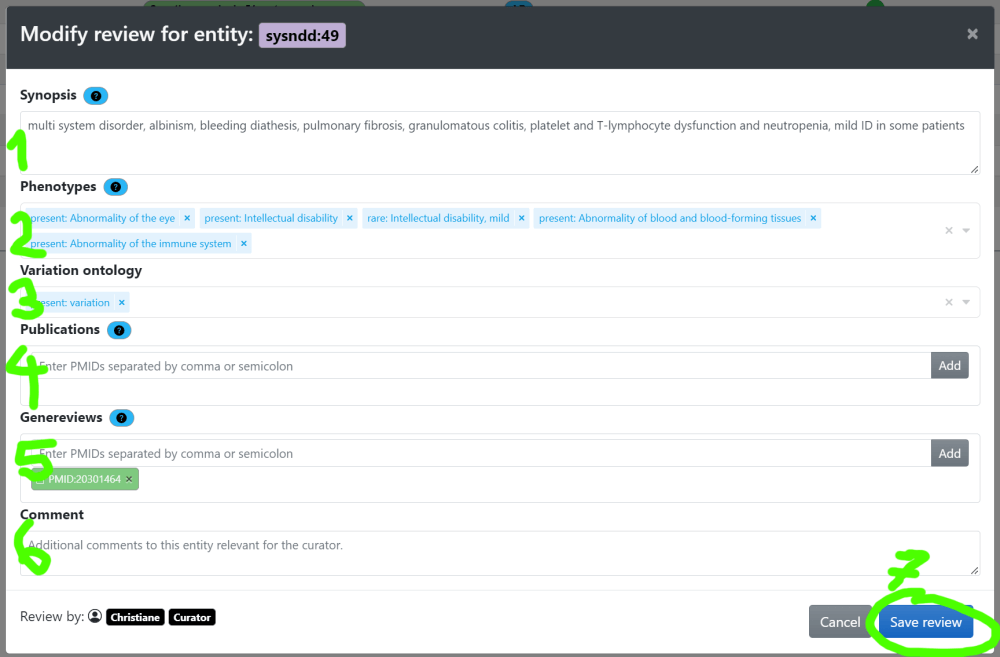
\includegraphics{./static/img/modal_modify_review.png}
\caption{Review page}
\end{figure}

These help instructions are:

\textbf{Synopsis}: Short summary for this disease entity. Please include information on: a) approximate number of patients described in literature, b) nature of reported variants, b) severity of intellectual disability, c) further phenotypic aspects (if possible with frequencies) d) any valuable further information (e.g.~genotype-phenotype correlations).

~~~~ Examples:

\begin{quote}
\emph{de novo} truncating or missense variants in \textgreater{} 20 individuals: variable ID (mild to severe), 50\% short stature and microcephaly, 30\% seizures, non-specific facial dysmorphism, variable cardiac and renal anomalies in some
\end{quote}

\begin{quote}
bi-allelic truncating variants in 7 individuals from 3 families: severe ID, microcephaly, seizures in 3/7, MRI anomalies
\end{quote}

\textbf{Phenotypes}: Add or remove associated phenotypes. Only phenotypes that occur in 20\% or more of affected individuals should be included. Please also include information on severity of ID where available and applicable.

\textbf{Publications}: No complete catalogue of entity-related literature required! If information in the clinical synopsis is not only based on OMIM entries, please include PMID of the article(s) used as a source for the clinical synopsis.

\textbf{GeneReviews}: Please add PMID for GeneReview article if available for this entity.

\textbf{Comment}: Additionally add information about your review potentially helpful to the curator approving the entity later.

\hypertarget{new-status-edit}{%
\subsubsection{New Status edit}\label{new-status-edit}}

In this window you can propose

\begin{itemize}
\tightlist
\item
  to change the entities association confidence category \textbf{(1)},
\item
  suggest it's overall removal \textbf{(2)},
\item
  add a comment for your change suggestions for the Curators to better understand the proposal \textbf{(3)} and
\item
  save your work \textbf{(4)}:
\end{itemize}

\begin{figure}
\centering
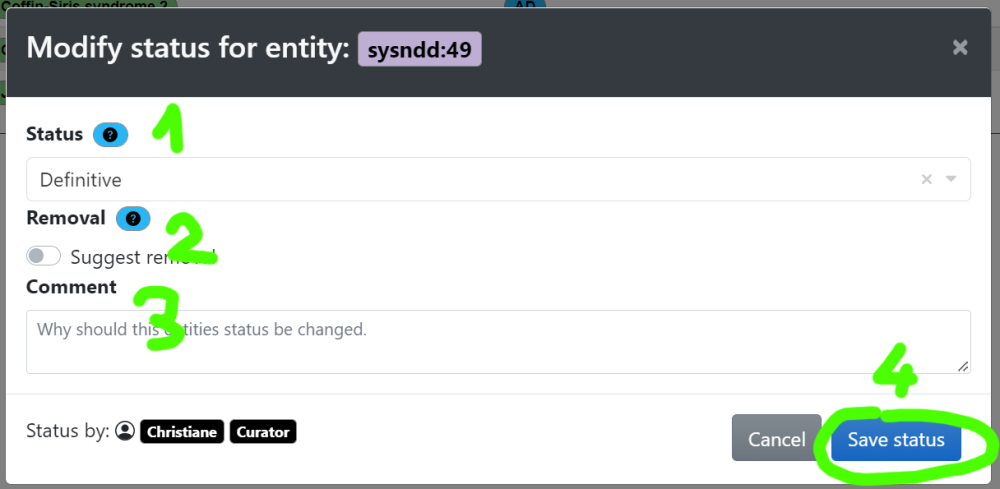
\includegraphics{./static/img/modal_modify_status.png}
\caption{Submit re-review modal}
\end{figure}

\hypertarget{submit-re-review}{%
\subsubsection{Submit Re-review}\label{submit-re-review}}

The last action window is just to confirm that you are satisfied with your work and would like to submit it for curation:

\begin{figure}
\centering
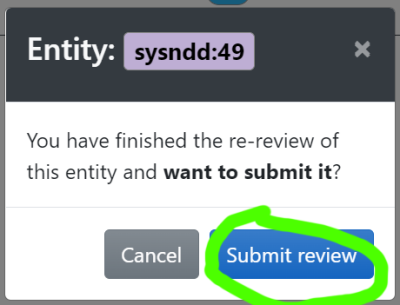
\includegraphics{./static/img/modal_submit_re-review.png}
\caption{Submit re-review modal}
\end{figure}

After clicking this button, the entity will disappear from your list. And you can proceed with the remaining entries until no entity is left in your list.

\hypertarget{re-review-curation}{%
\subsection{Re-review curation}\label{re-review-curation}}

\hypertarget{definitive-association-status}{%
\subsubsection{Definitive association status}\label{definitive-association-status}}

\begin{enumerate}
\def\labelenumi{\arabic{enumi}.}
\tightlist
\item
  Check if category 1 (``Definitive'') is correct or shift status to category 2 (``Moderate'') or 3 (``Limited''), where appropriate
\item
  Check and revise gene-related entities regarding diseases/inheritance patterns (ID and non-ID disorders) --\textgreater{} non-ID disorders will not go into any of the categories but will be tagged with ``n.a.'' (not applicable)
\item
  Check and revise associated phenotypes: select HPO terms from the list, only use HPO term if this specific aspect is present in approximately \textgreater= 20\% of patients. Please also check and revise severity of ID using HPO terms. If ID is very variable, select all appropriate ID terms (e.g.~severe, moderate, mild, borderline)
\item
  Check references (OMIM, PMID, GeneReviews). References do not have to be complete but should be sufficient to give a good impression on the mutational and clinical spectrum. Add references where it would add to the picture.
\item
  Check and revise clinical synopsis: it does not have to contain everything that is known but should give a short and comprehensive picture on:
\end{enumerate}

\begin{itemize}
\tightlist
\item
  which data the gene and disease category were chosen on and
\item
  the molecular and clinical picture.
\end{itemize}

Please include information on:

\begin{enumerate}
\def\labelenumi{\alph{enumi})}
\tightlist
\item
  approximate number of patients described in literature,
\item
  nature of reported variants,
\item
  severity of intellectual disability,
\item
  further phenotypic aspects (if possible with frequencies),
\item
  any valuable further information (e.g.~genotype-phenotype correlations)
\end{enumerate}

Examples:

\begin{quote}
\emph{de novo} truncating or missense variants in \textgreater{} 20 individuals: variable ID (mild to severe), 50\% short stature and microcephaly, 30\% seizures, non-specific facial dysmorphism, variable cardiac and renal anomalies in some
\end{quote}

\begin{quote}
bi-allelic truncating variants in 7 individuals from 3 families: severe ID, microcephaly, seizures in 3/7, MRI anomalies
\end{quote}

\hypertarget{moderate-and-limited-association-status}{%
\subsubsection{Moderate and Limited association status}\label{moderate-and-limited-association-status}}

\begin{itemize}
\tightlist
\item
  Check if inclusion criteria for candidate genes are still fulfilled or if it should be deleted from the list (``Refuted'')
\item
  Check if candidate status is still correct and sort it into Category 2 (``Moderate'') and 3 (``Limited'') (or reclassify to 1 (``Definitive''), if applicable)
\item
  Check, if associated phenotype still fits
\item
  Check, if references are correct, if there is any new published information and modify clinical synopsis where appropriate
\item
  Clinical synopsis can be very short for candidate genes
\item
  no associated phenotypes (HPO terms) and frequencies are needed for candidate genes, but could be helpful
\end{itemize}

Examples:

\begin{quote}
\emph{de novo} missense variants in 2 individuals: autism, ID in 50\%
\end{quote}

\begin{quote}
bi-allelic missense variant in 2 affected individuals from 1 family: moderate ID, MRI anomalies
\end{quote}

\hypertarget{refuted-association-status}{%
\subsubsection{Refuted association status}\label{refuted-association-status}}

\begin{itemize}
\tightlist
\item
  Check if there is current evidence against this gene association (e.g.~few truncating variants described in old publications before gnomAD constrain scores and the gene now has a pLI of 0; genes reported in a family with later report of another cause etc.)
\end{itemize}

  \bibliography{sysndd.bib}

\end{document}
